\documentclass[11pt]{article}
\title{Laporan Tugas Basisdata II}
\author{Hanif Amrullah / 1184020}
\usepackage{graphicx}


\begin{document}
\maketitle

\section{Langkah-Langkah Membuat Aplikasi dengan Oracle}
Berikut langkah-langkah membuat aplikasi apex.
\begin{enumerate}

\item
pertama-tama pastikan anda sudah membuat datanya terlebih dahulu dengan \textit{Excel} seperti contoh dibawah :
\begin{figure}[h]
        \centerline{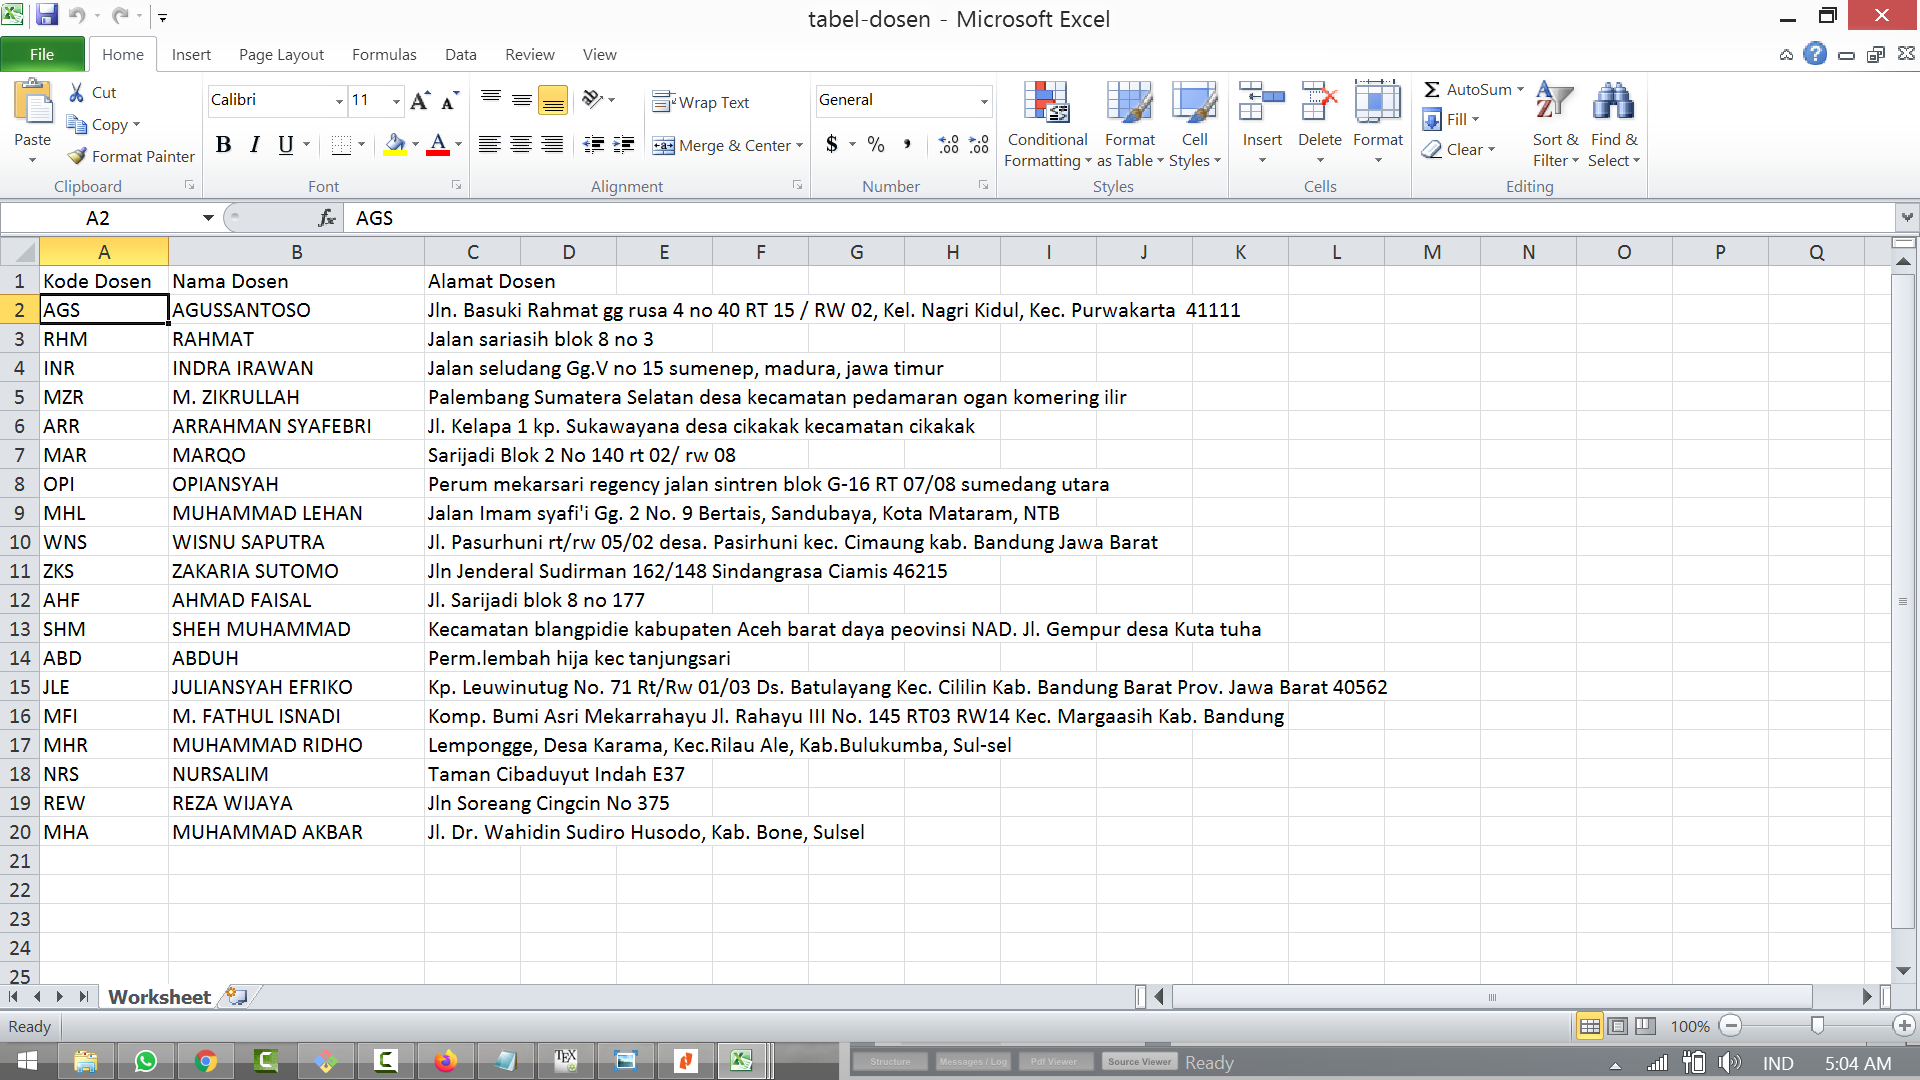
\includegraphics[scale=0.1]{img/t1.png}}
        \caption{}
        \centering
	\label{langkah1}
	\end{figure}
\begin{figure}[h]
        \centerline{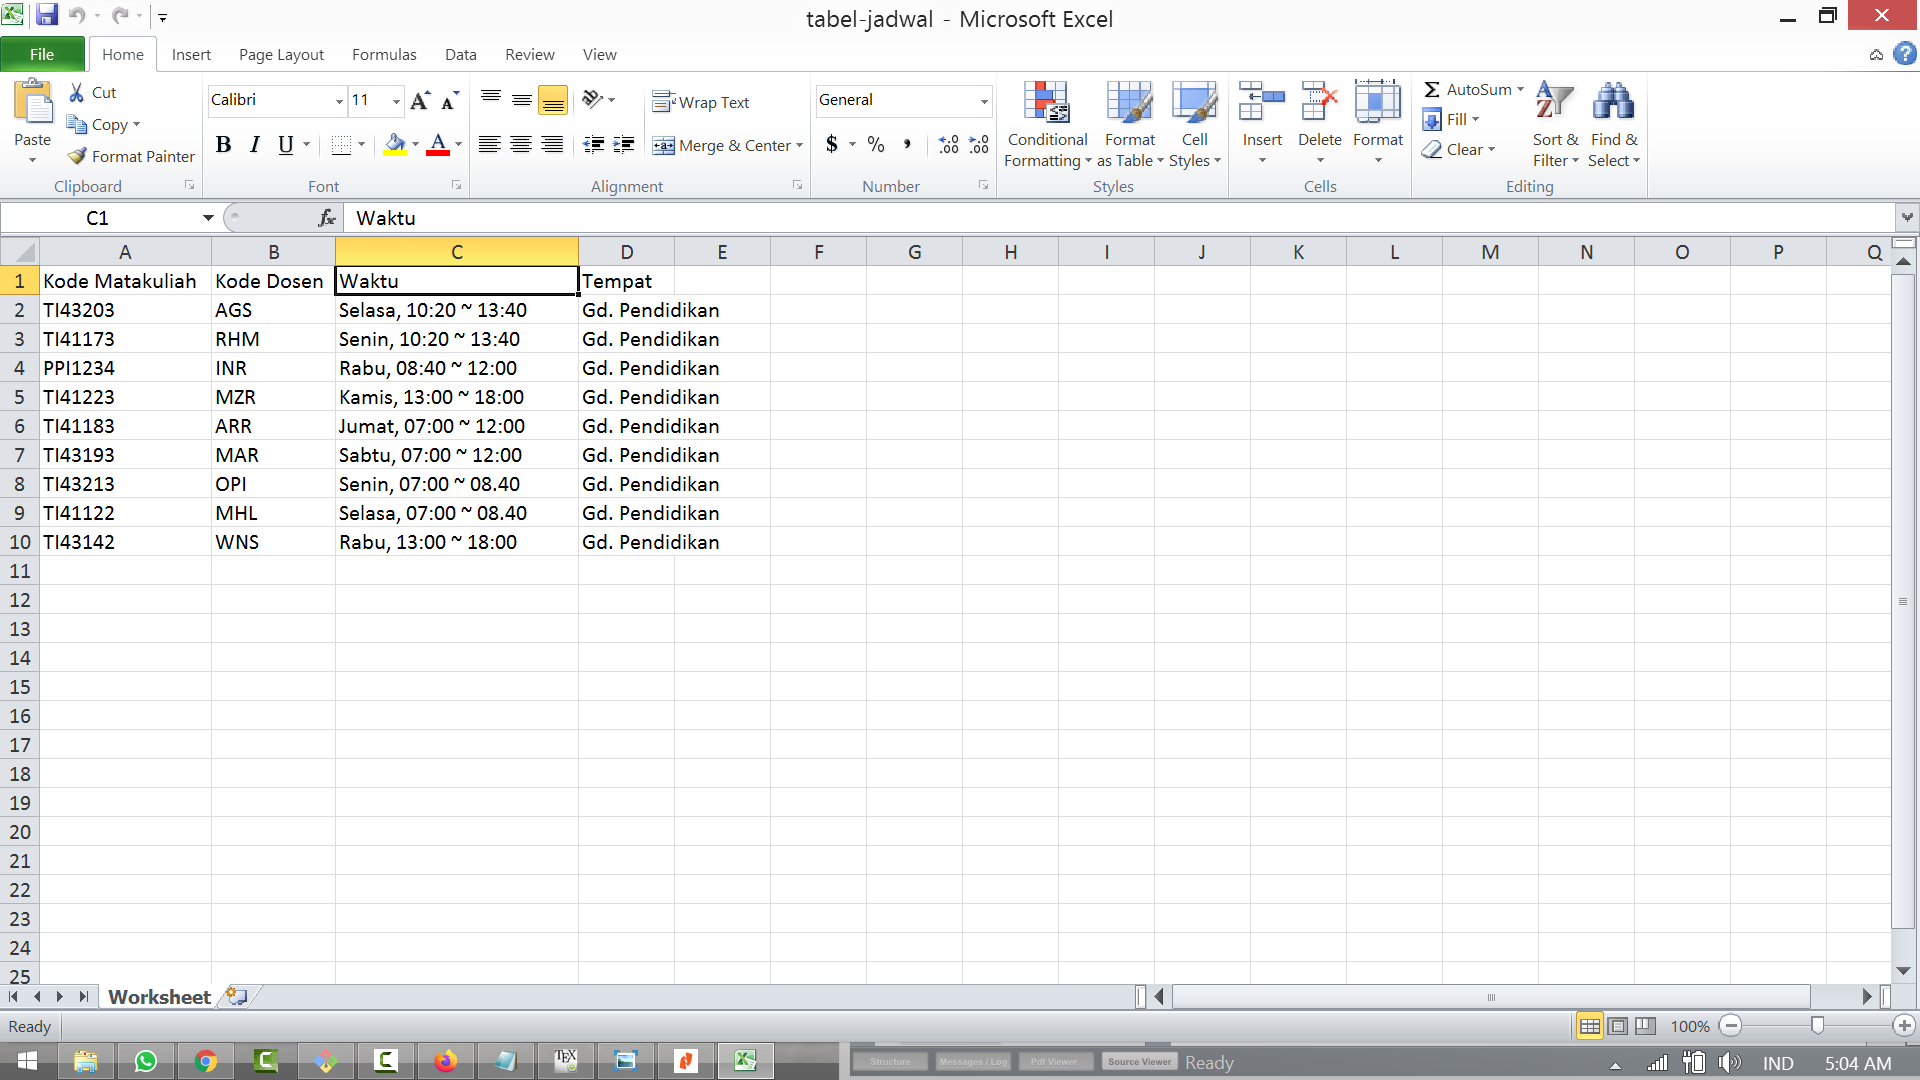
\includegraphics[scale=0.1]{img/t2.png}}
        \caption{}
        \centering
	\label{langkah2}
	\end{figure}

\newpage
\begin{figure}[h]
        \centerline{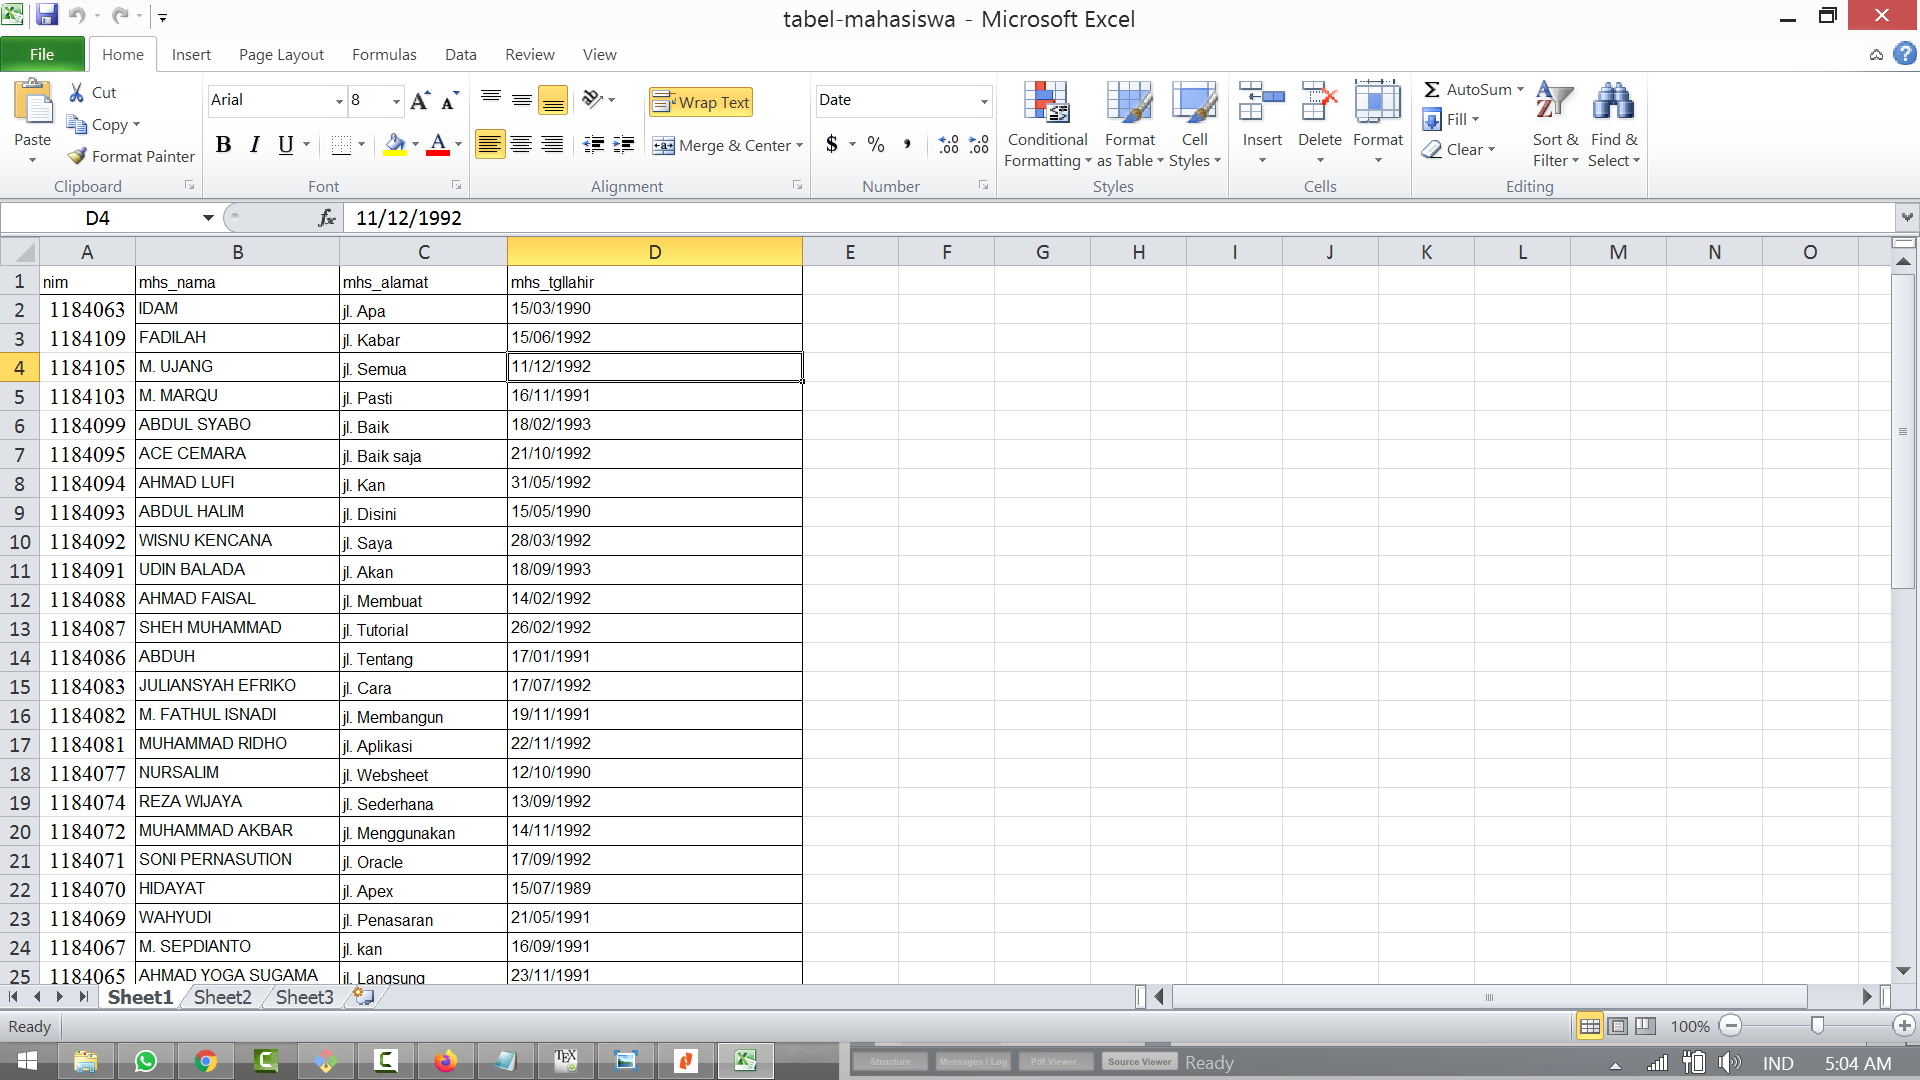
\includegraphics[scale=0.1]{img/t3.png}}
        \caption{}
        \centering
	\label{langkah3}
	\end{figure}
\begin{figure}[h]
        \centerline{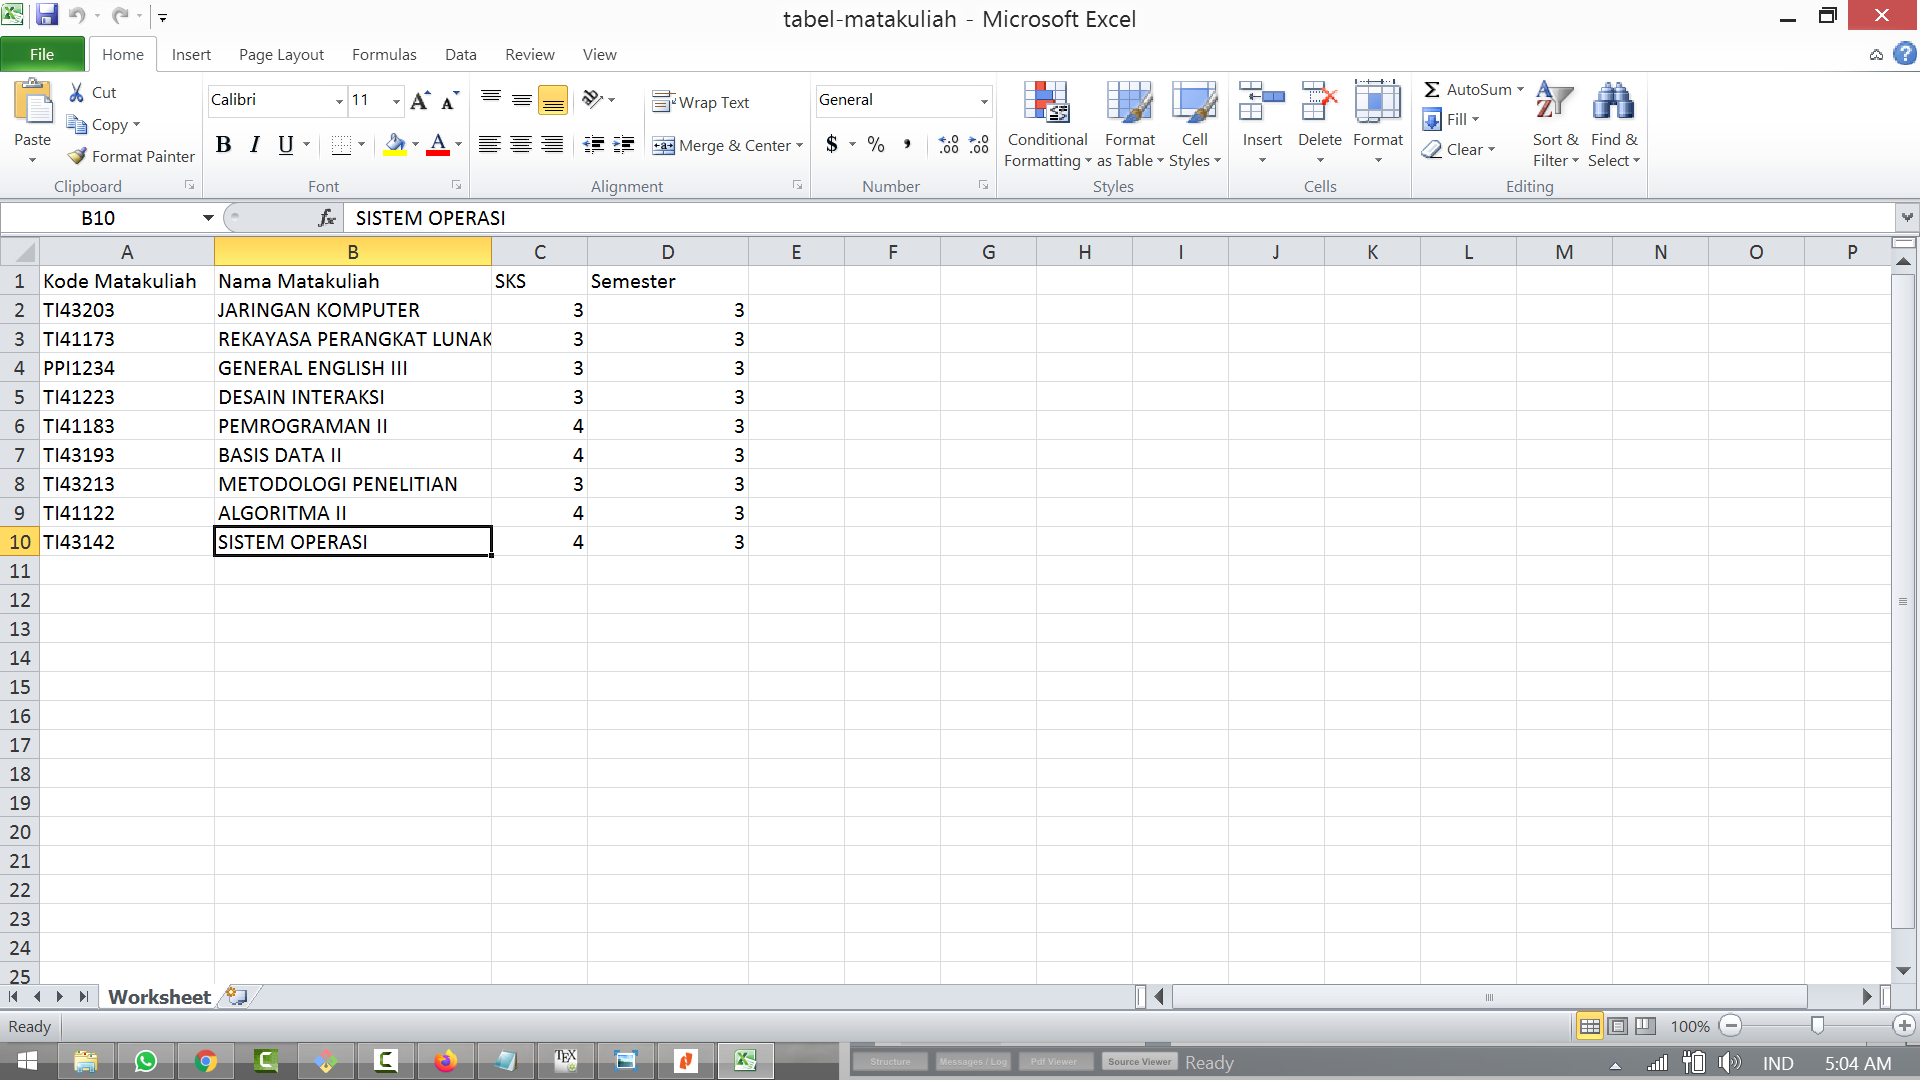
\includegraphics[scale=0.1]{img/t4.png}}
        \caption{}
        \centering
	\label{langkah4}
	\end{figure}

\newpage
\begin{figure}[h]
        \centerline{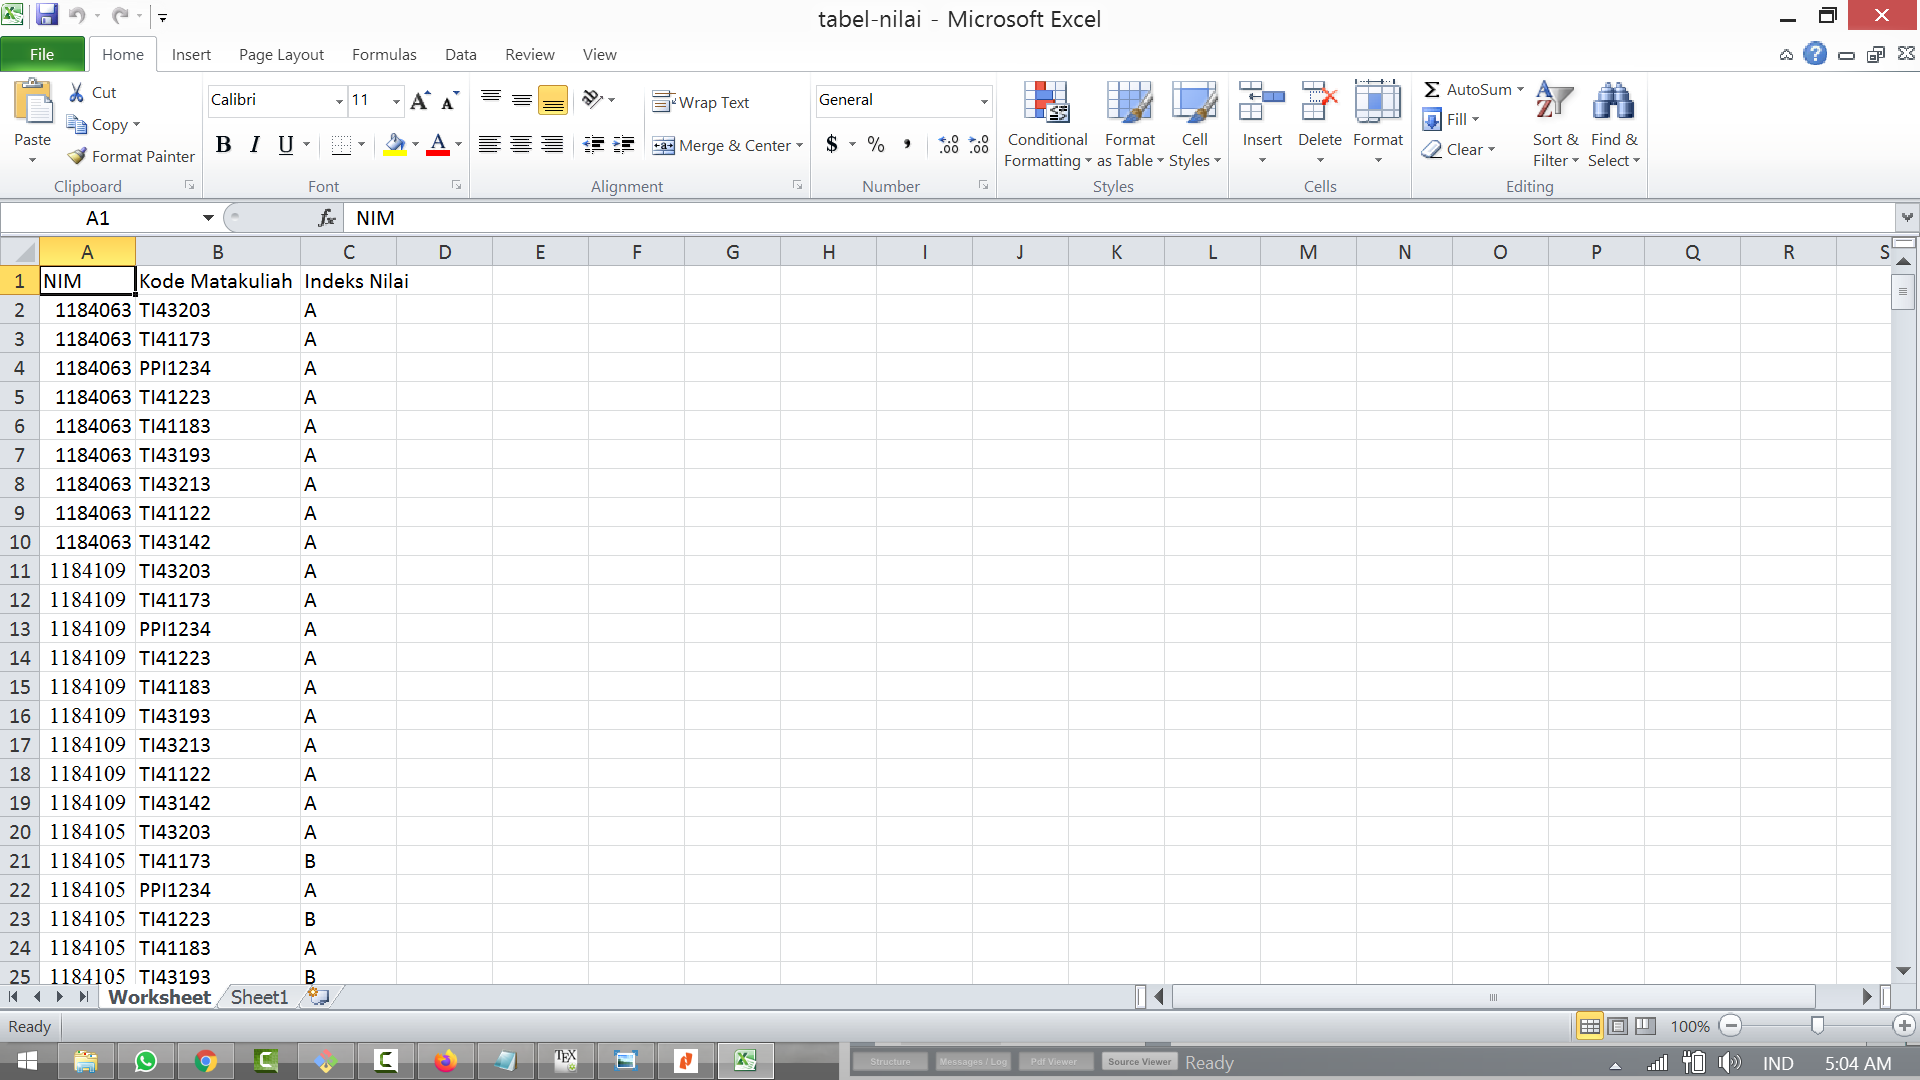
\includegraphics[scale=0.1]{img/t5.png}}
        \caption{}
        \centering
	\label{langkah5}
	\end{figure}

\newpage
\item 
Kunjungi website oracle apex "https://apex.oracle.com/en/" dan klik sign in
	\begin{figure}[h]
		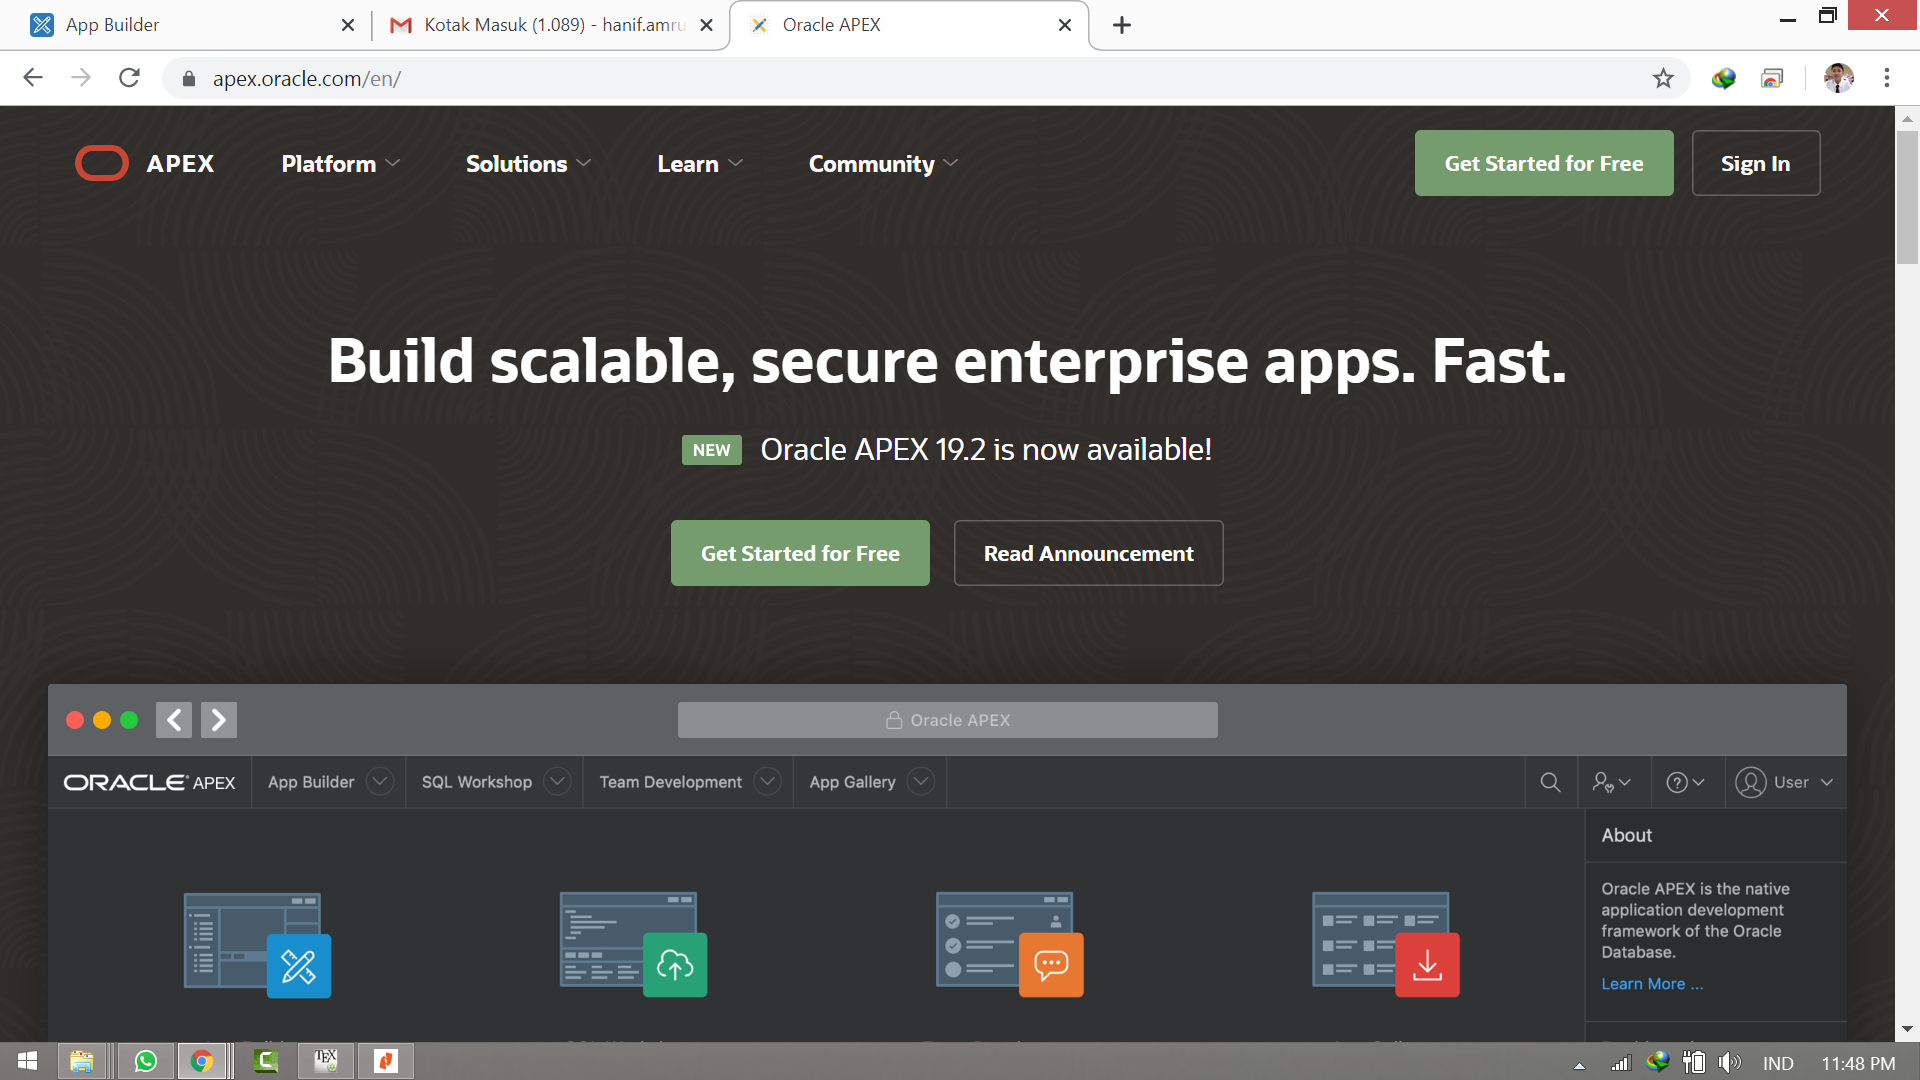
\includegraphics[scale= 0.1]{img/web.png}
		\centering
		\caption{}
	\label{langkah6}
	\end{figure}

\item isi WorkSpace,Username, Passwoard
	\begin{figure}[h]
        \centerline{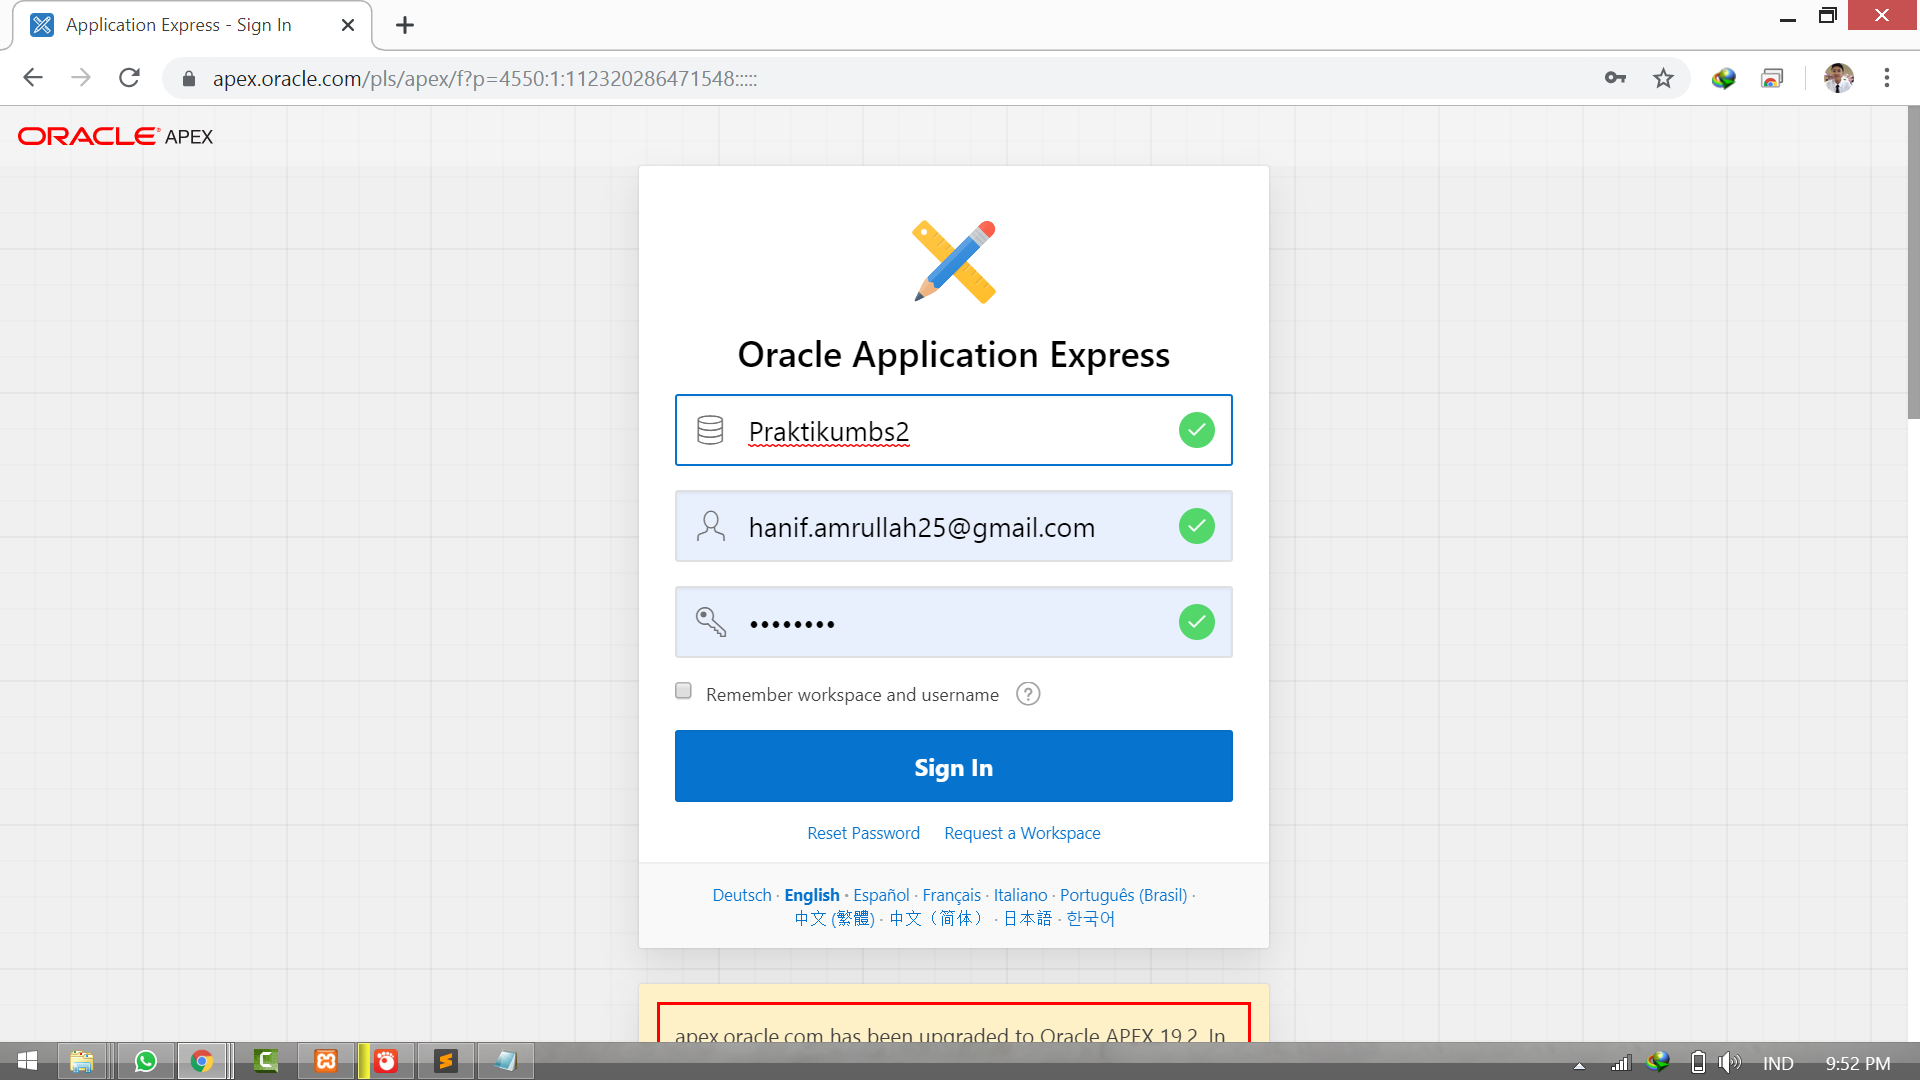
\includegraphics[scale=0.1]{img/1.png}}
        \caption{}
        \centering
	\label{langkah7}
	\end{figure}

\newpage
\item Klik \textbf{App Builder}
	\begin{figure}[h]
        \centerline{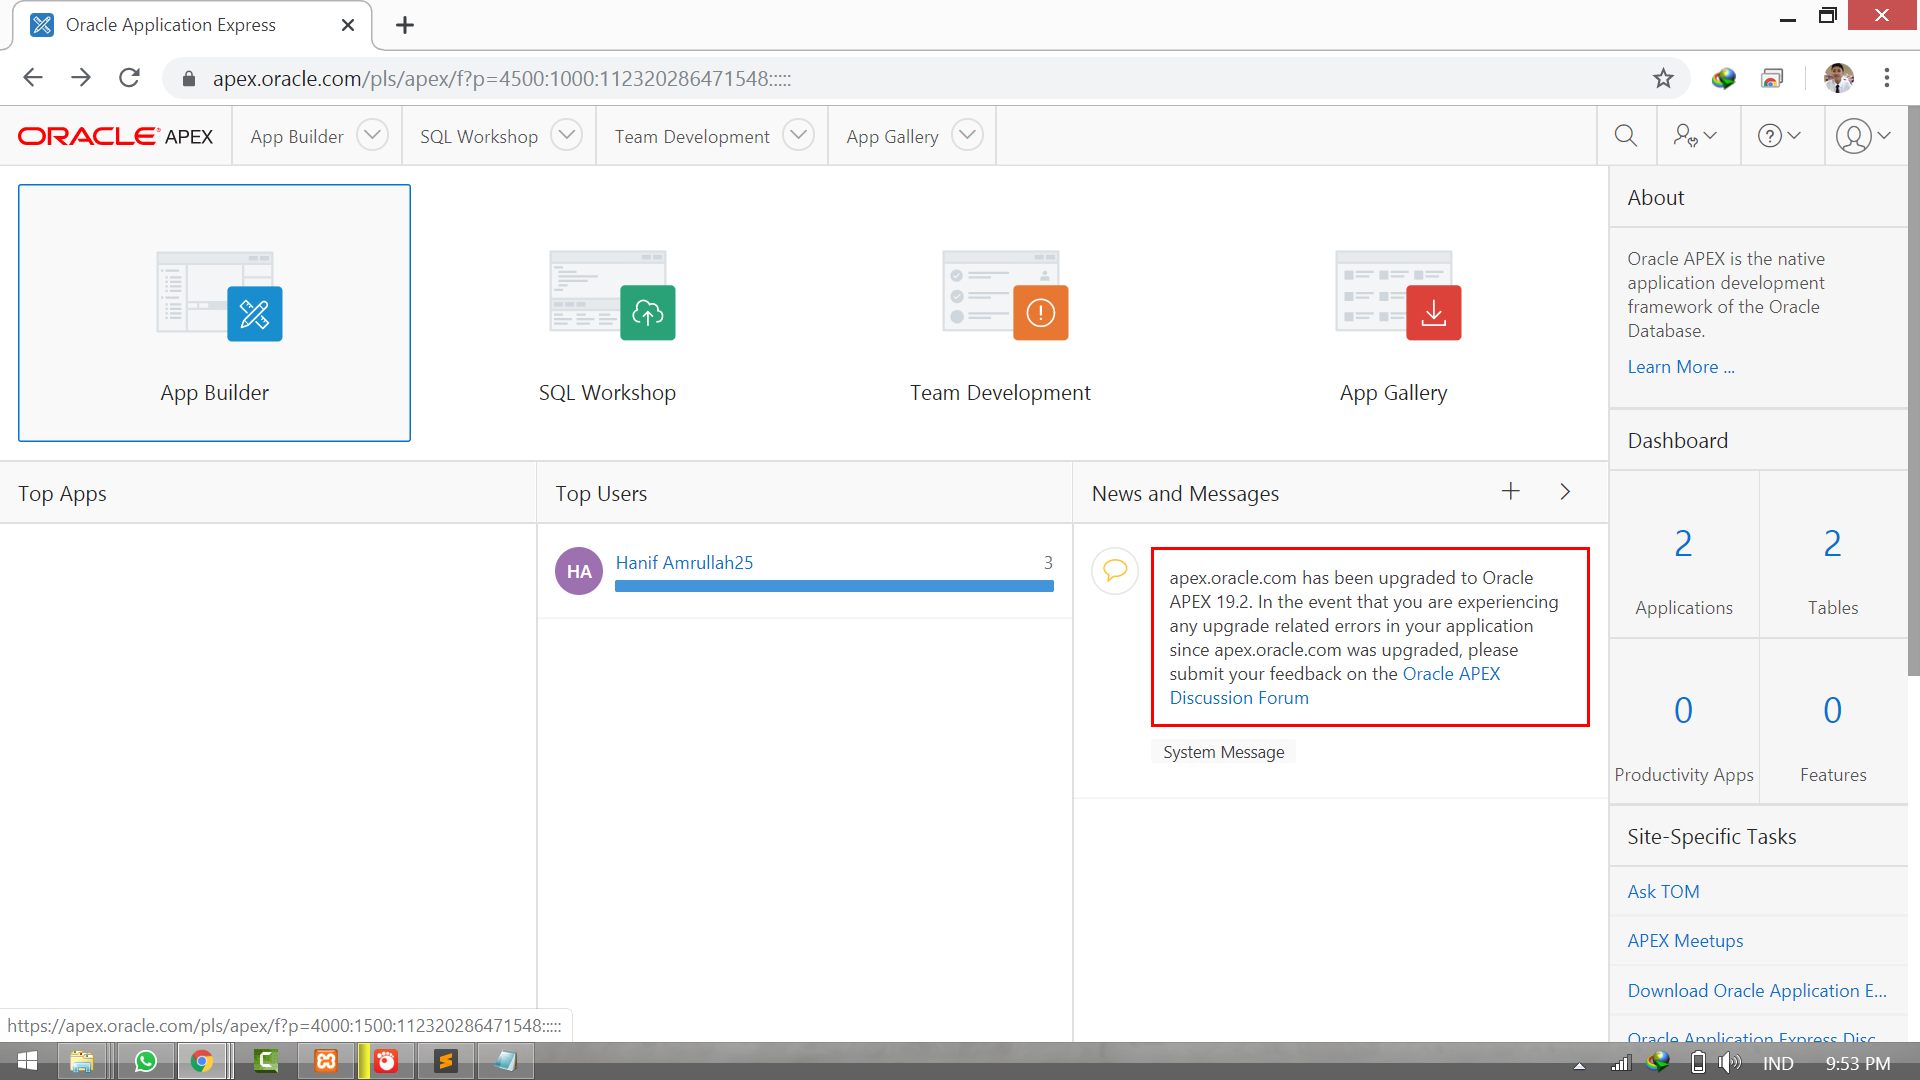
\includegraphics[scale=0.1]{img/2.png}}
        \centering
        \caption{}
		\label{langkah8}
		\end{figure}


\item klik \textbf{Create}
	\begin{figure}[h]
        \centerline{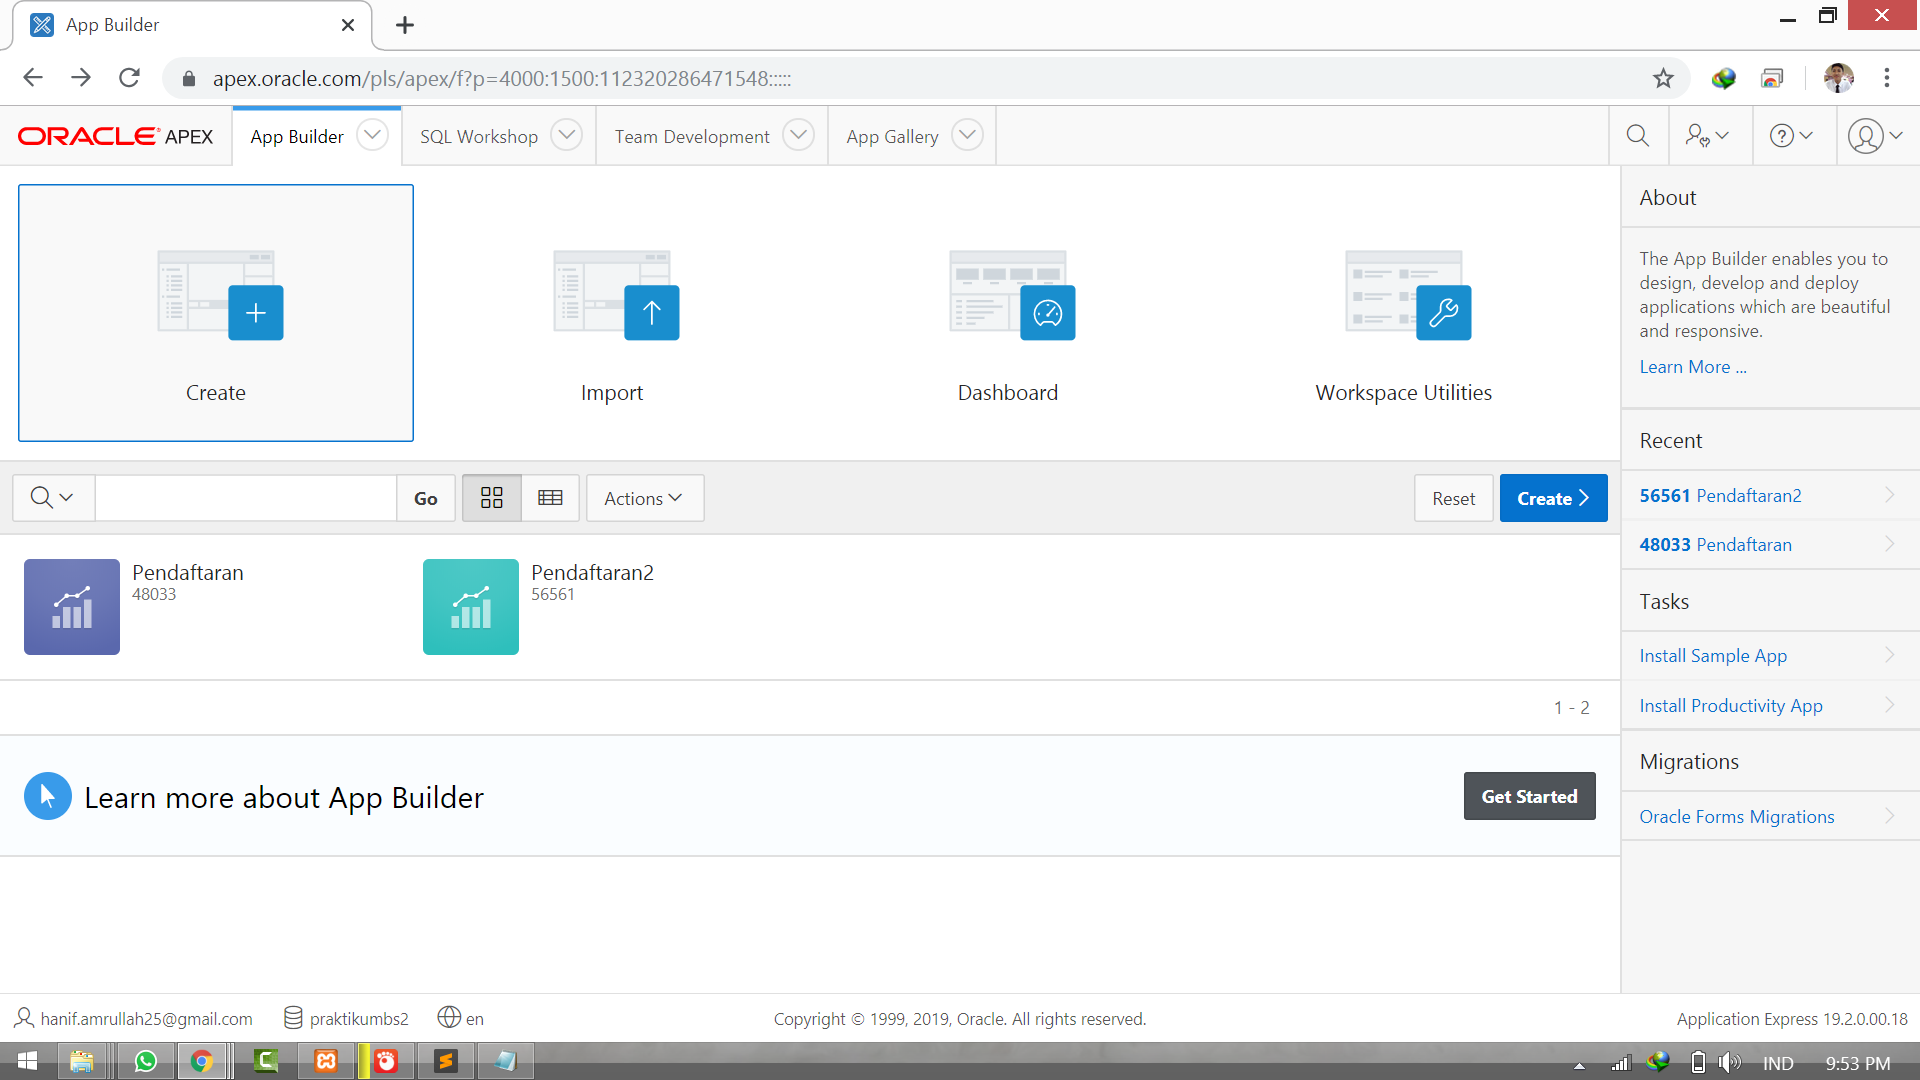
\includegraphics[scale=0.1]{img/3.png}}
        \centering
        \caption{}
		\label{langkah9}
		\end{figure}

\newpage
\item klik Form A File
	\begin{figure}[h]
        \centerline{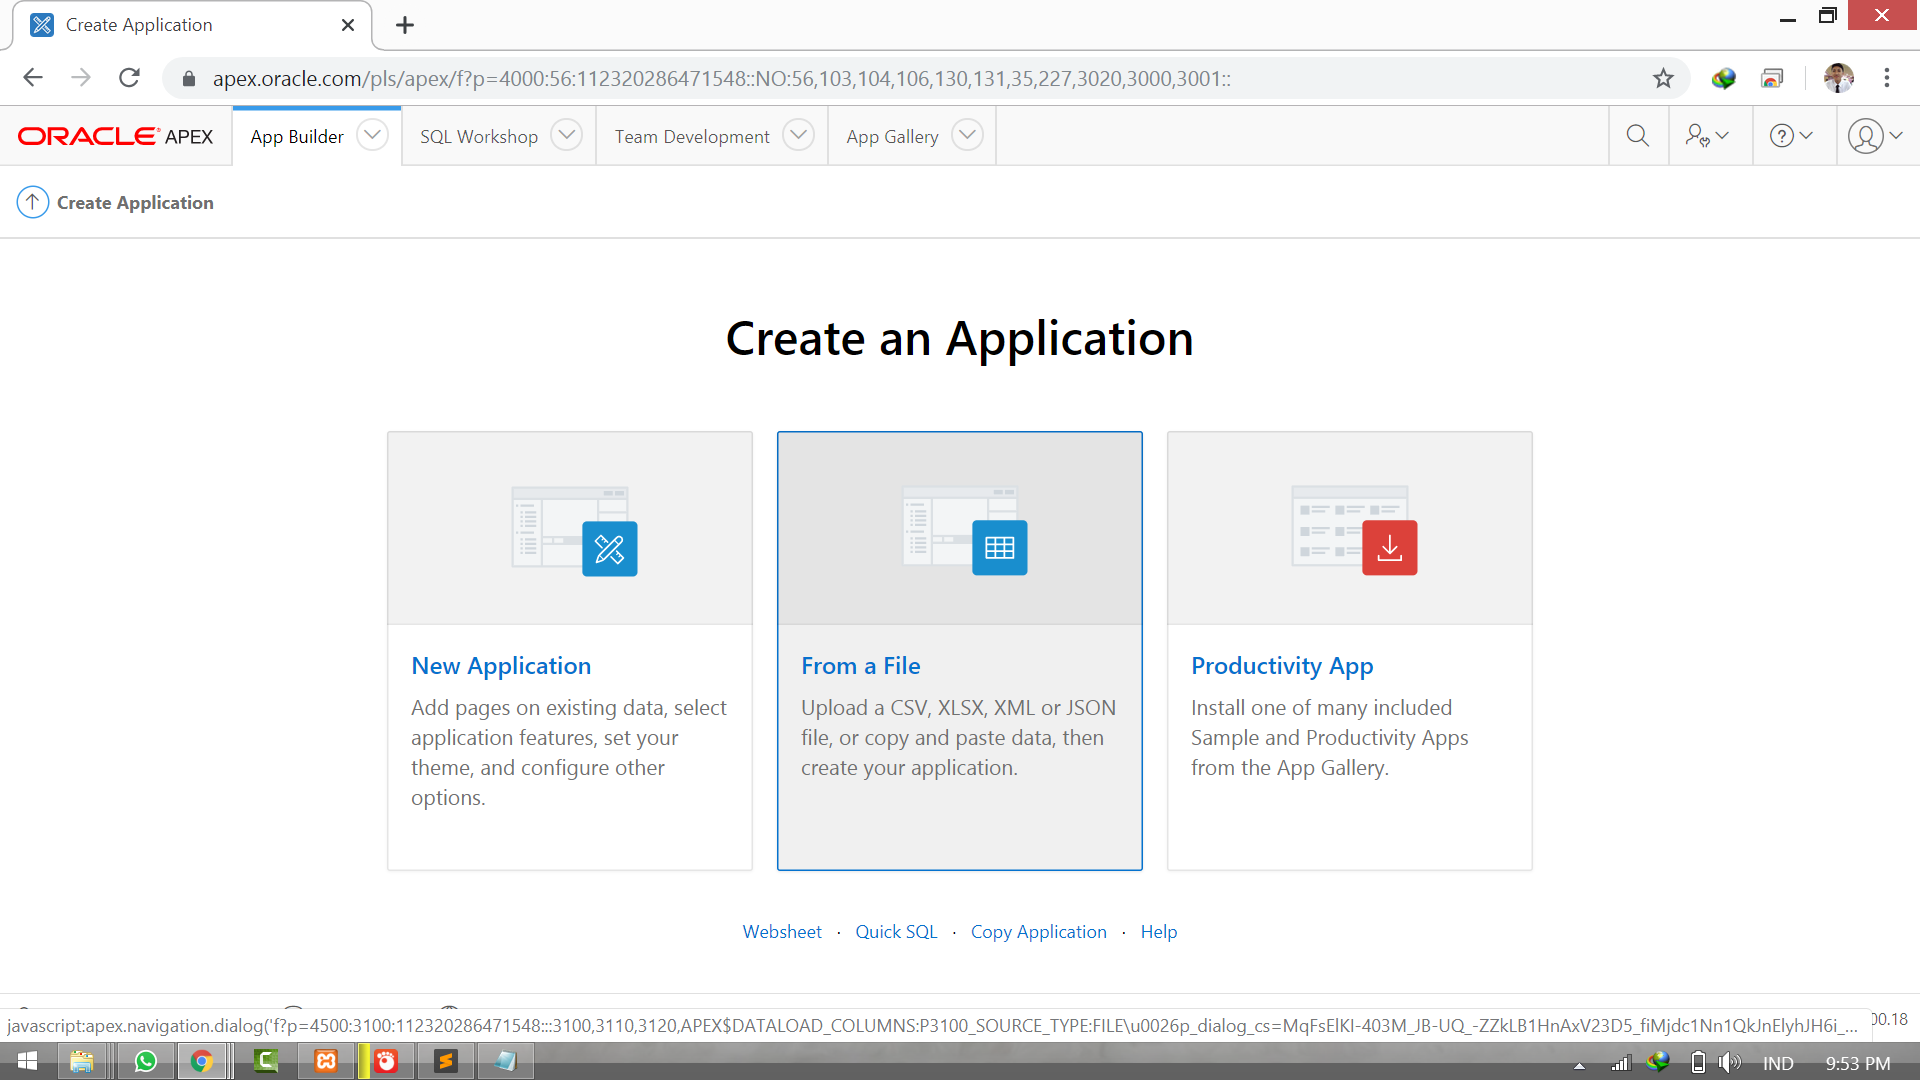
\includegraphics[scale=0.1]{img/4.png}}
        \centering
        \caption{}
		\label{langkah10}
	\end{figure}


\item pilih file tabel excel
	\begin{figure}[h]
        \centerline{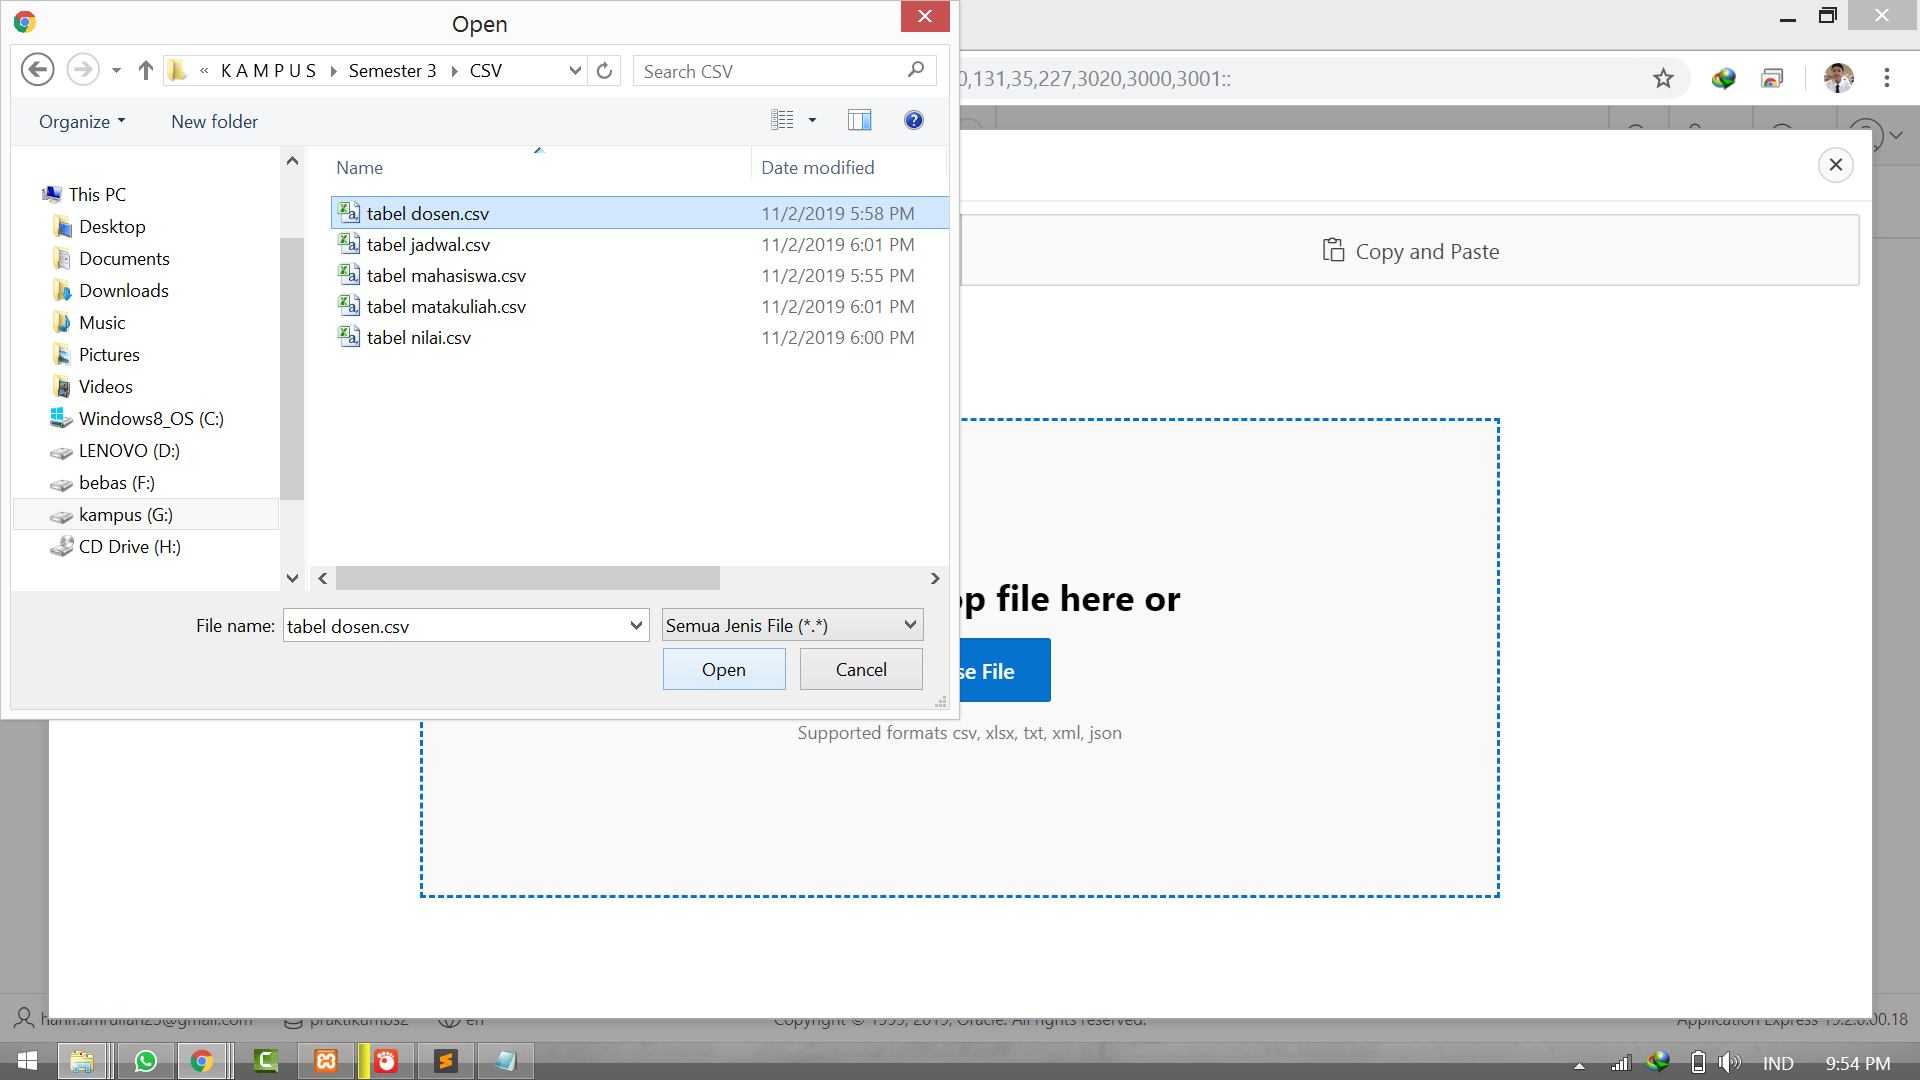
\includegraphics[scale=0.1]{img/5.png}}
        \centering
        \caption{}
		\label{langkah11}
	\end{figure}

\newpage
\item isi nama tabel di bagian \textbf{Table Name}, lalu klik \textbf{configura} untuk mengecek ada yang error
	\begin{figure}[h]
        \centerline{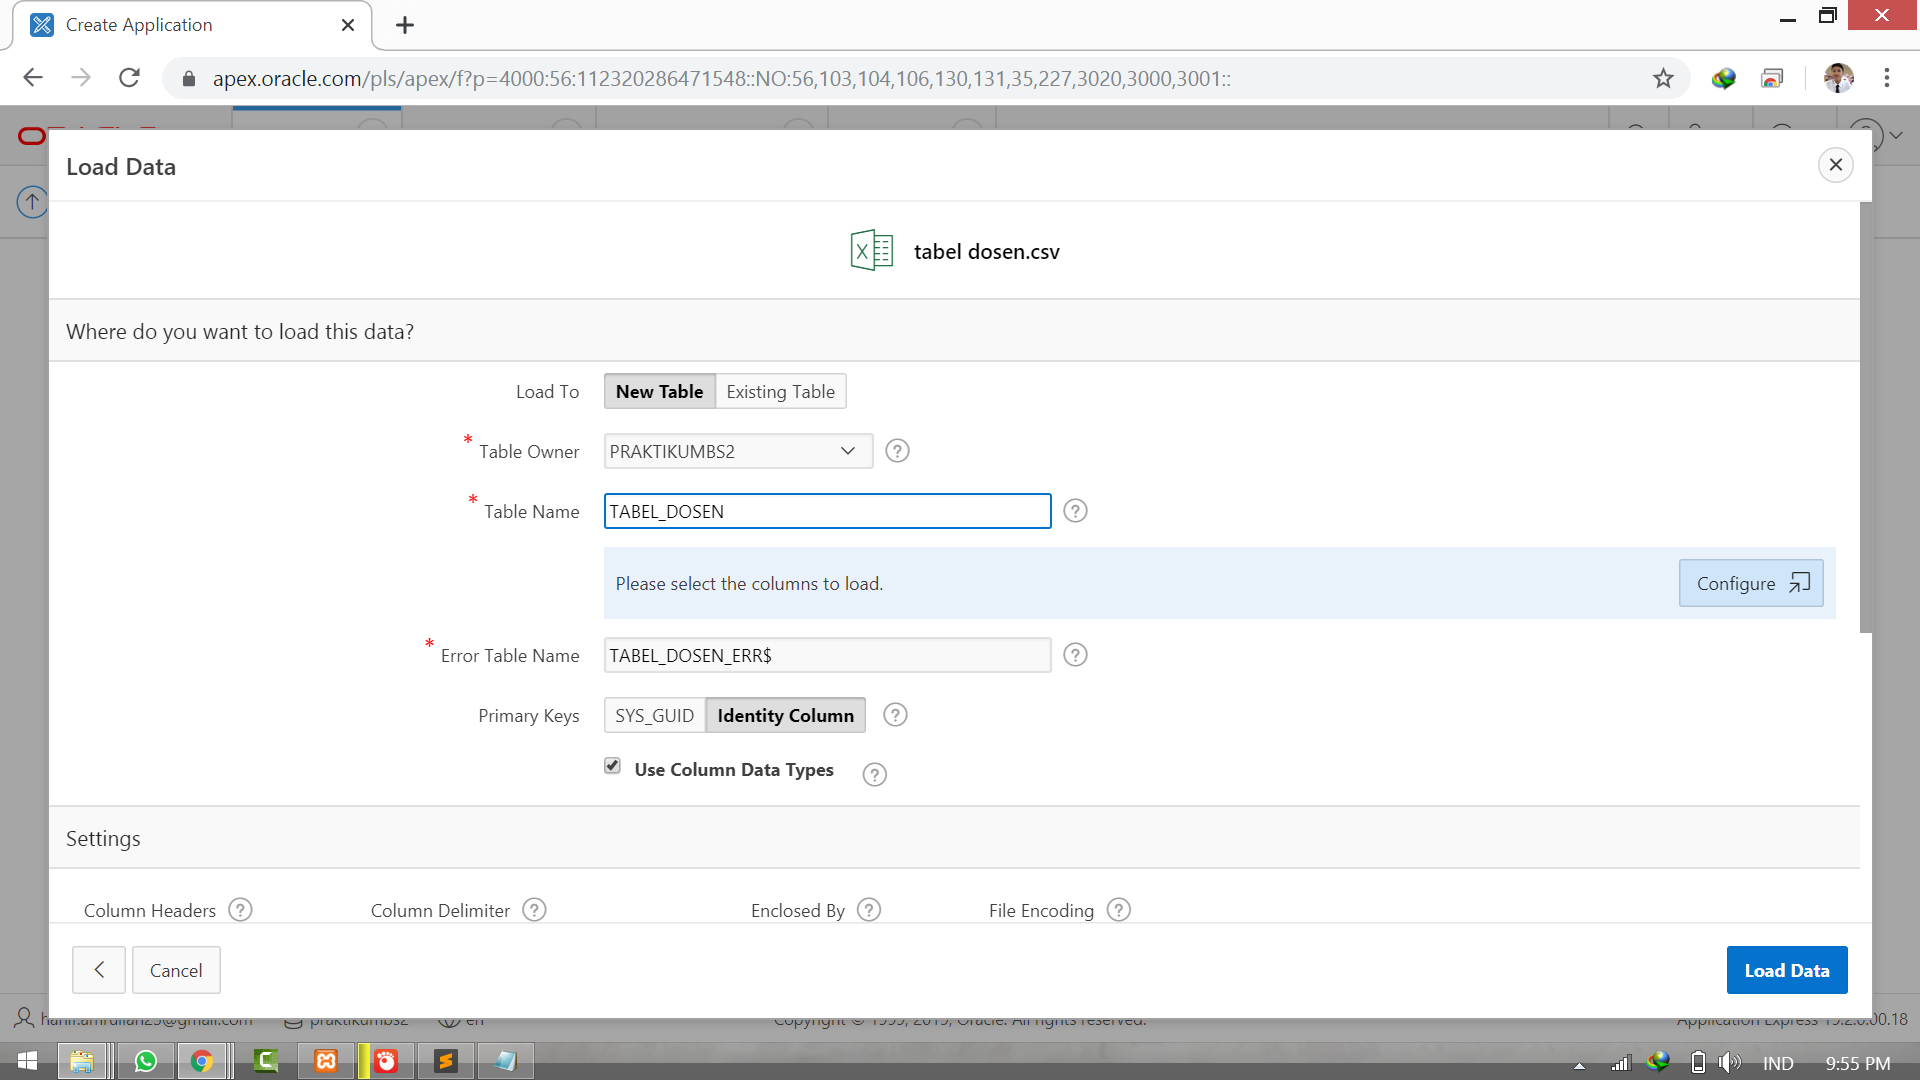
\includegraphics[scale=0.1]{img/6.png}}
        \centering
        \caption{}
		\label{langkah12}
	\end{figure}
	

\item klik \textbf{save change} apabila tidak ada error
	\begin{figure}[h]
        \centerline{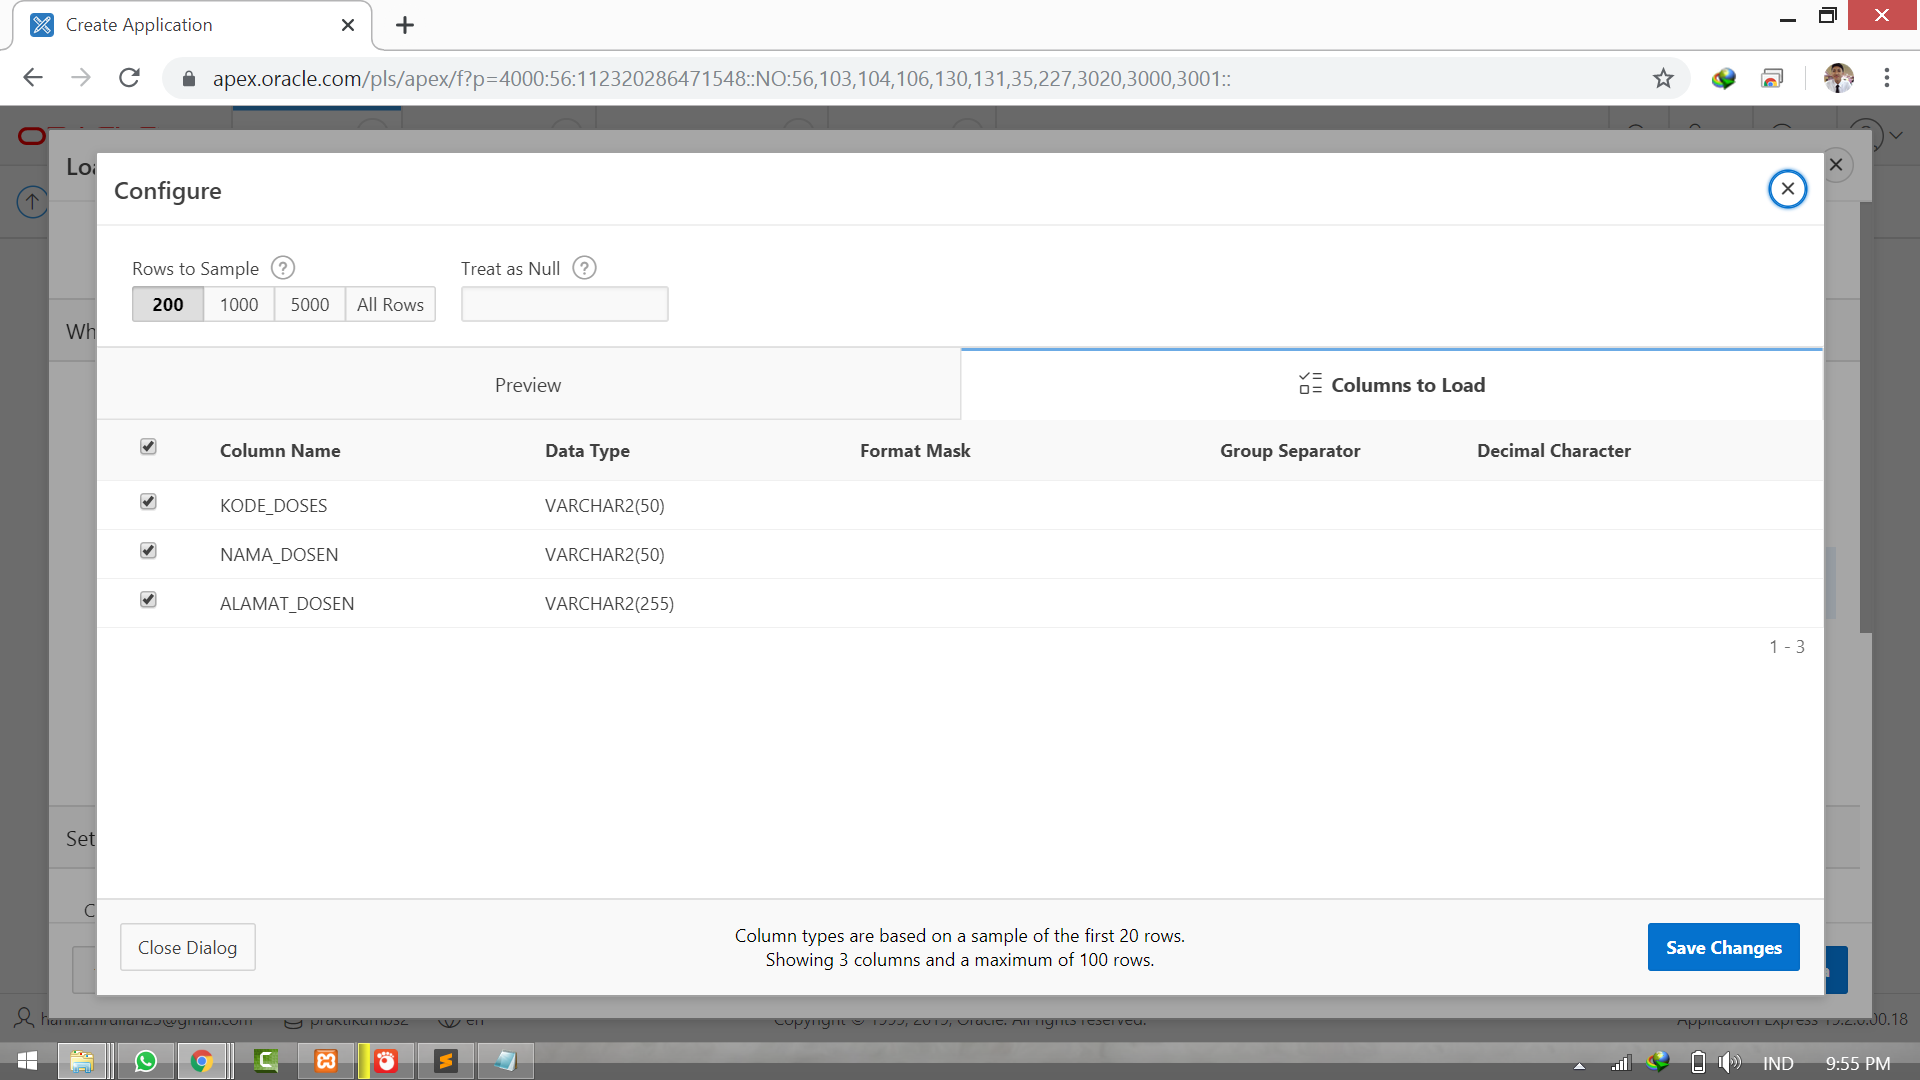
\includegraphics[scale=0.1]{img/7.png}}
        \centering
        \caption{}
		\label{langkah13}
	\end{figure}

\newpage	
\item klik \textbf{load data}
	\begin{figure}[h]
        \centerline{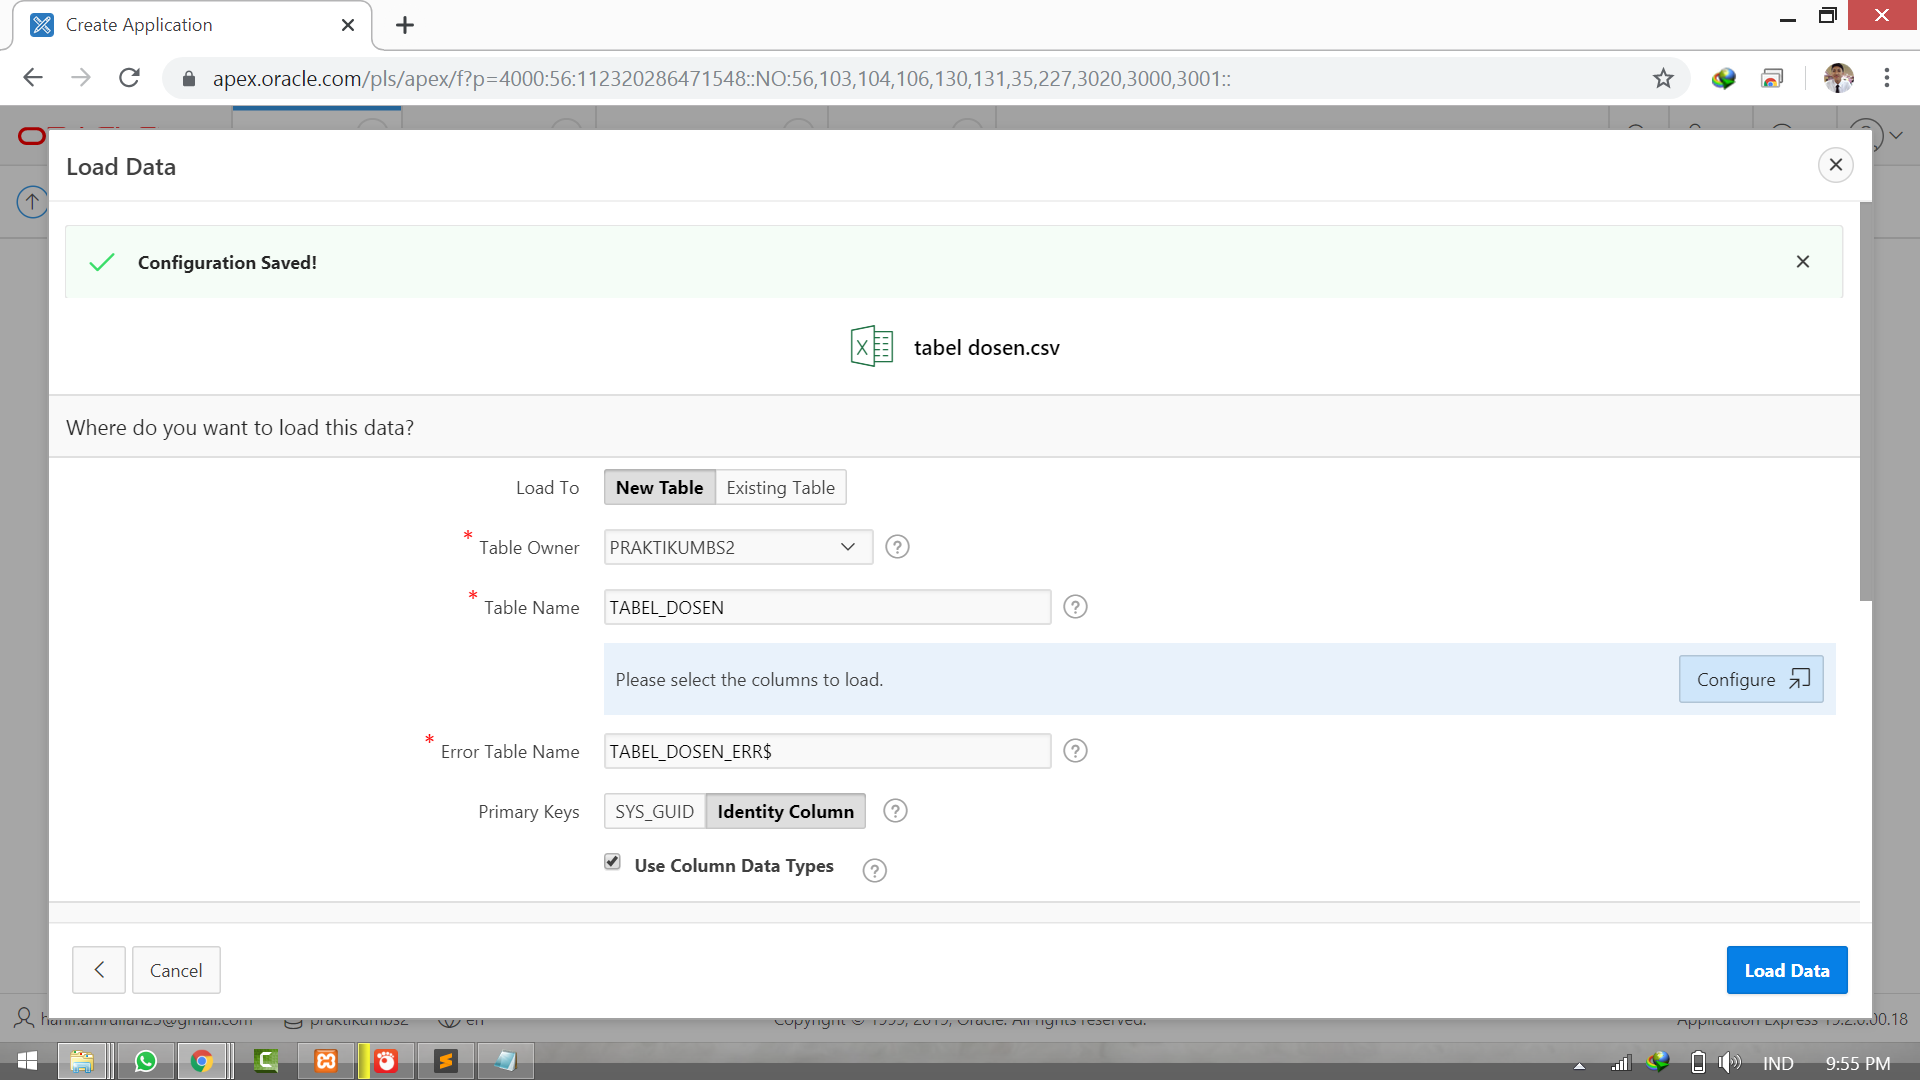
\includegraphics[scale=0.1]{img/8.png}}
        \centering
        \caption{}
		\label{langkah14}
	\end{figure}
	
\item klik \textbf{Create Application}
	\begin{figure}[h]
        \centerline{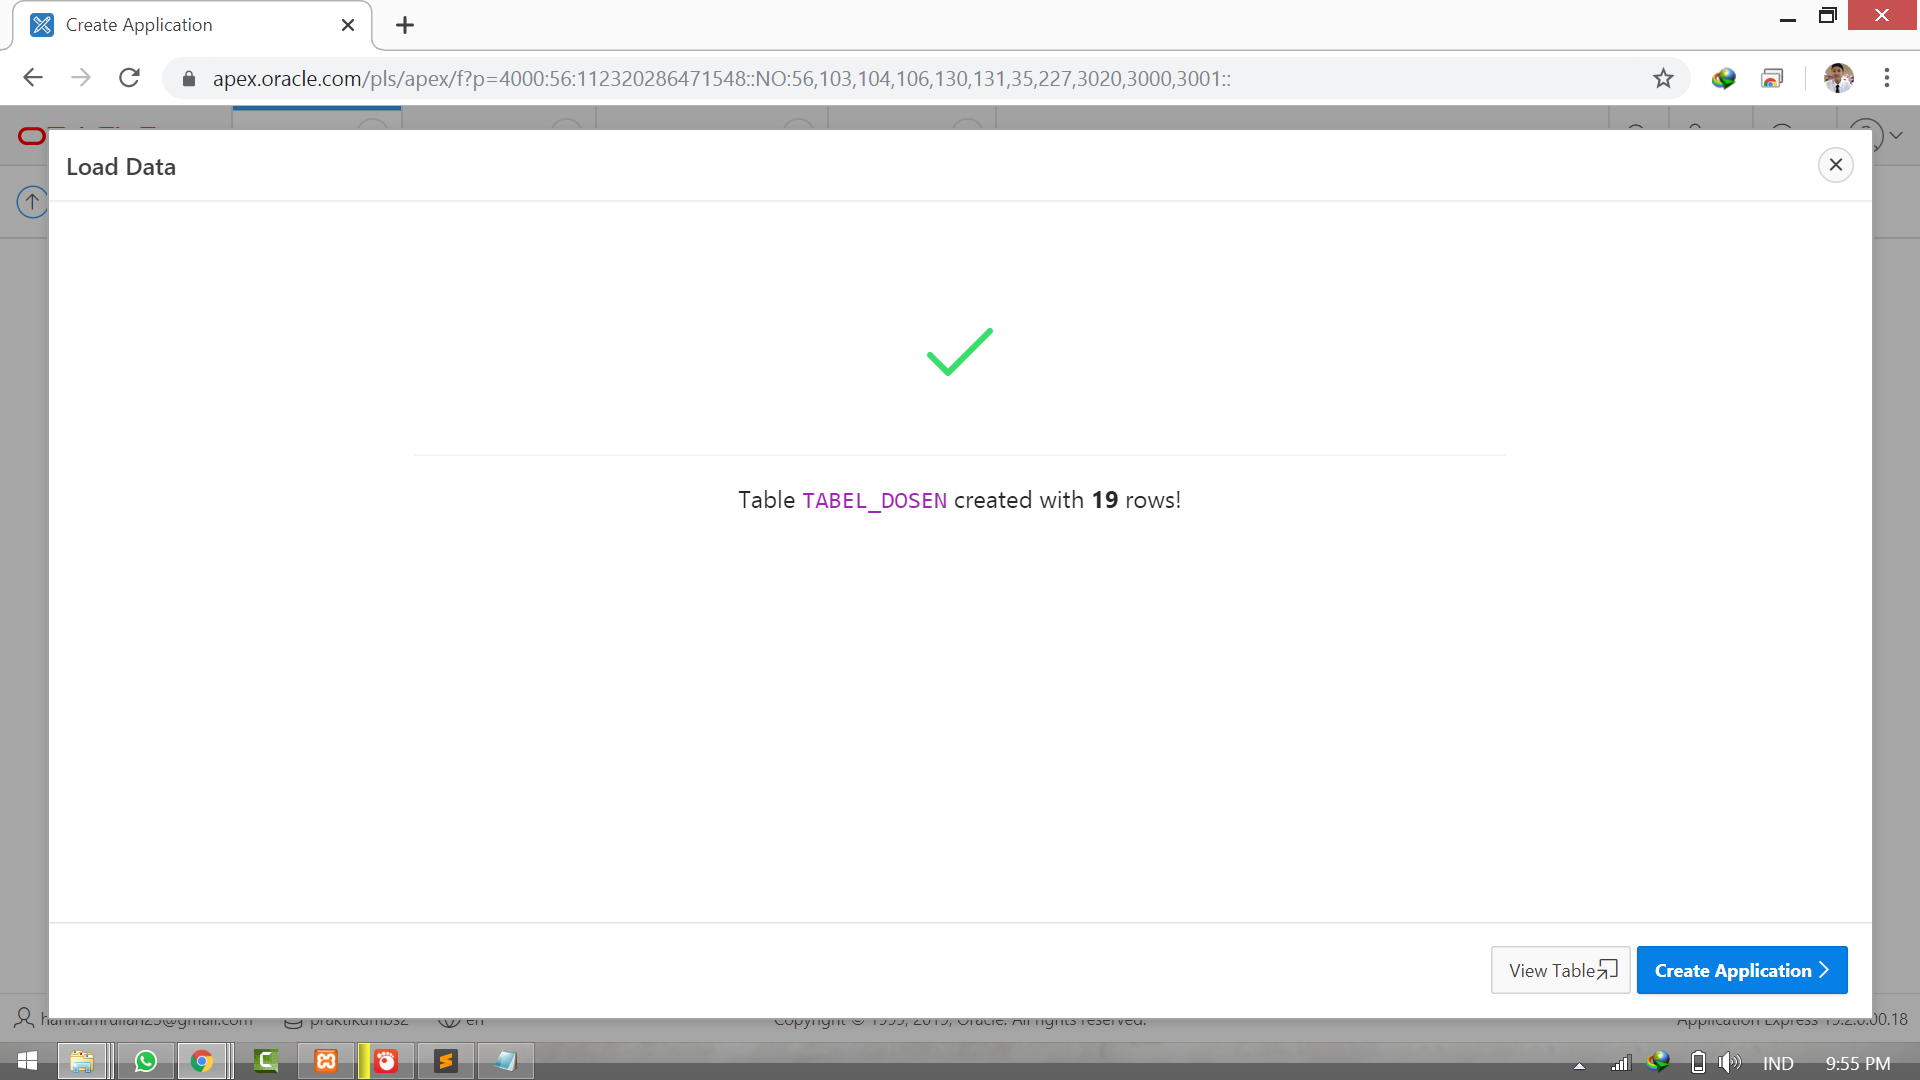
\includegraphics[scale=0.1]{img/9.png}}
        \centering
        \caption{}
		\label{langkah15}
	\end{figure}

\newpage	
\item scroll kebawah, klik \textbf{Create Application}
	\begin{figure}[h]
        \centerline{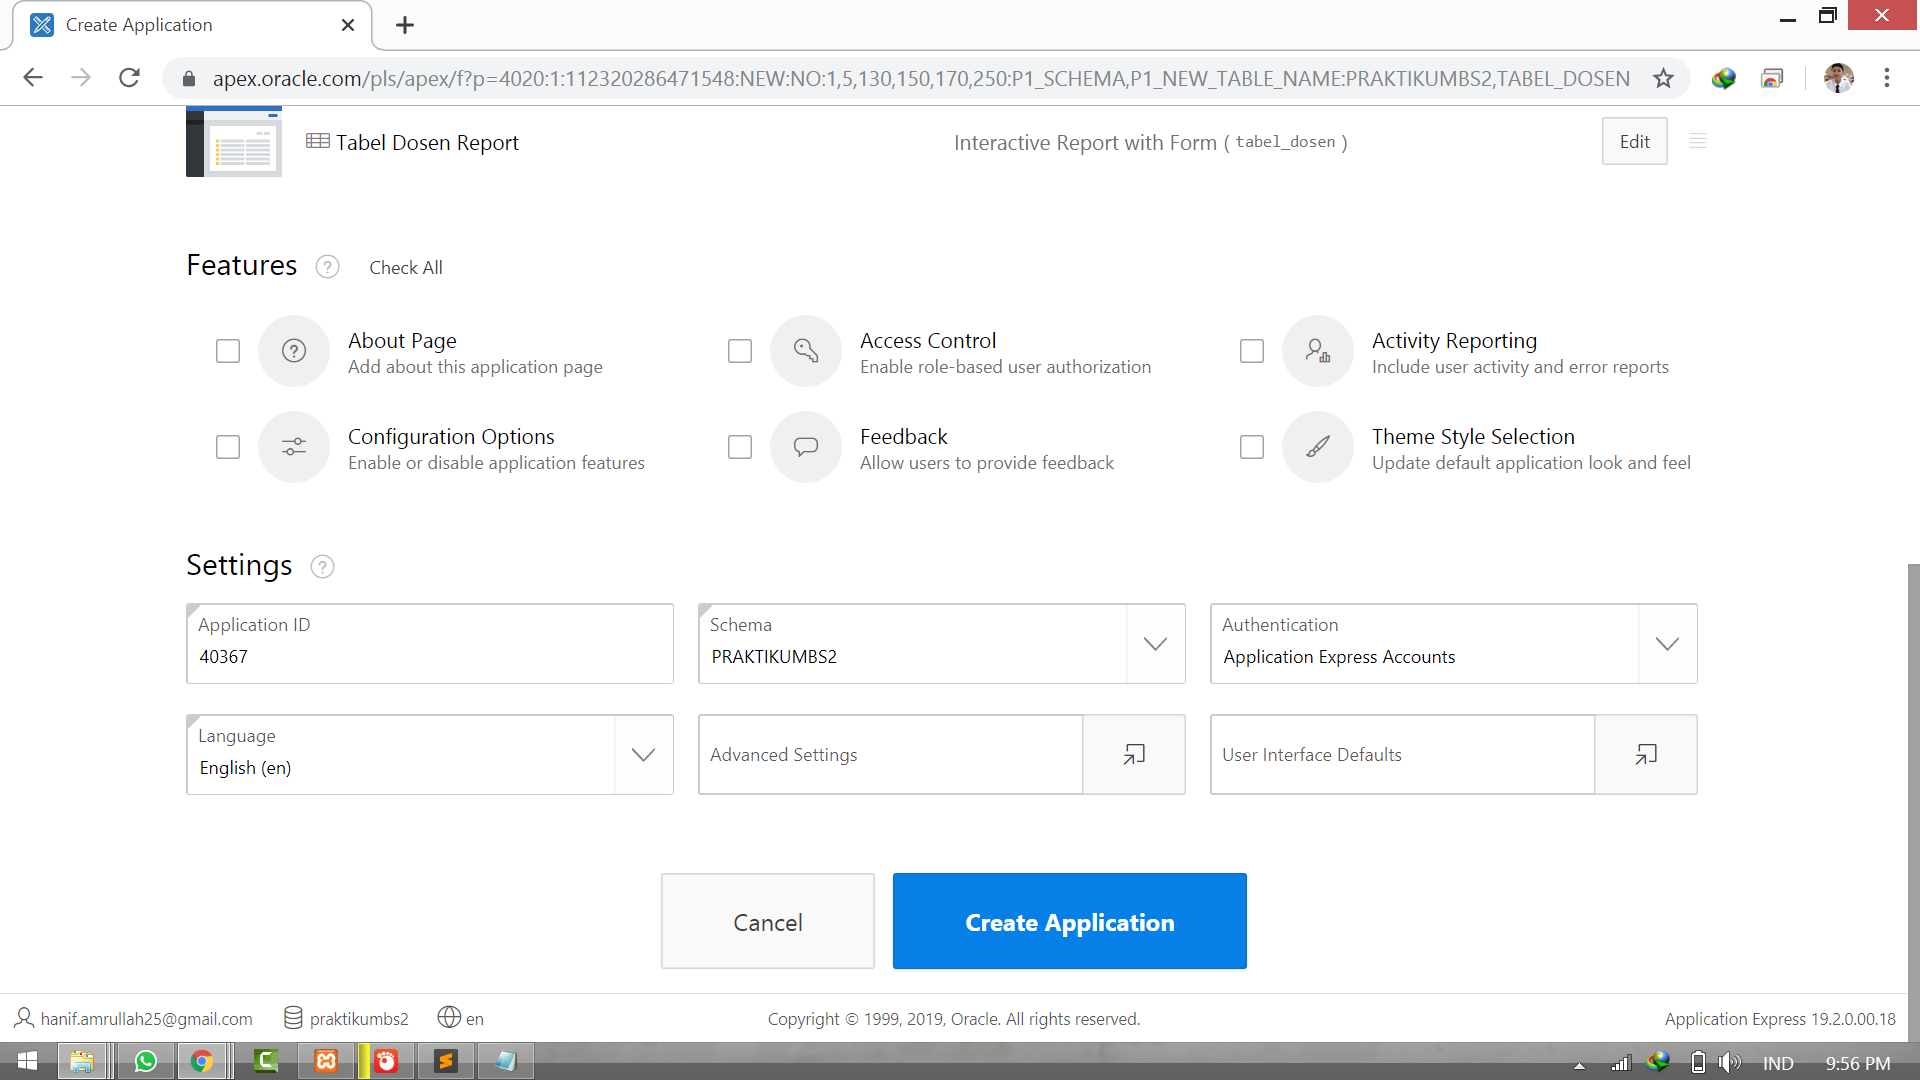
\includegraphics[scale=0.1]{img/10.png}}
        \centering
        \caption{}
		\label{langkah16}
	\end{figure}
	
\item tunggu proses
	\begin{figure}[h]
        \centerline{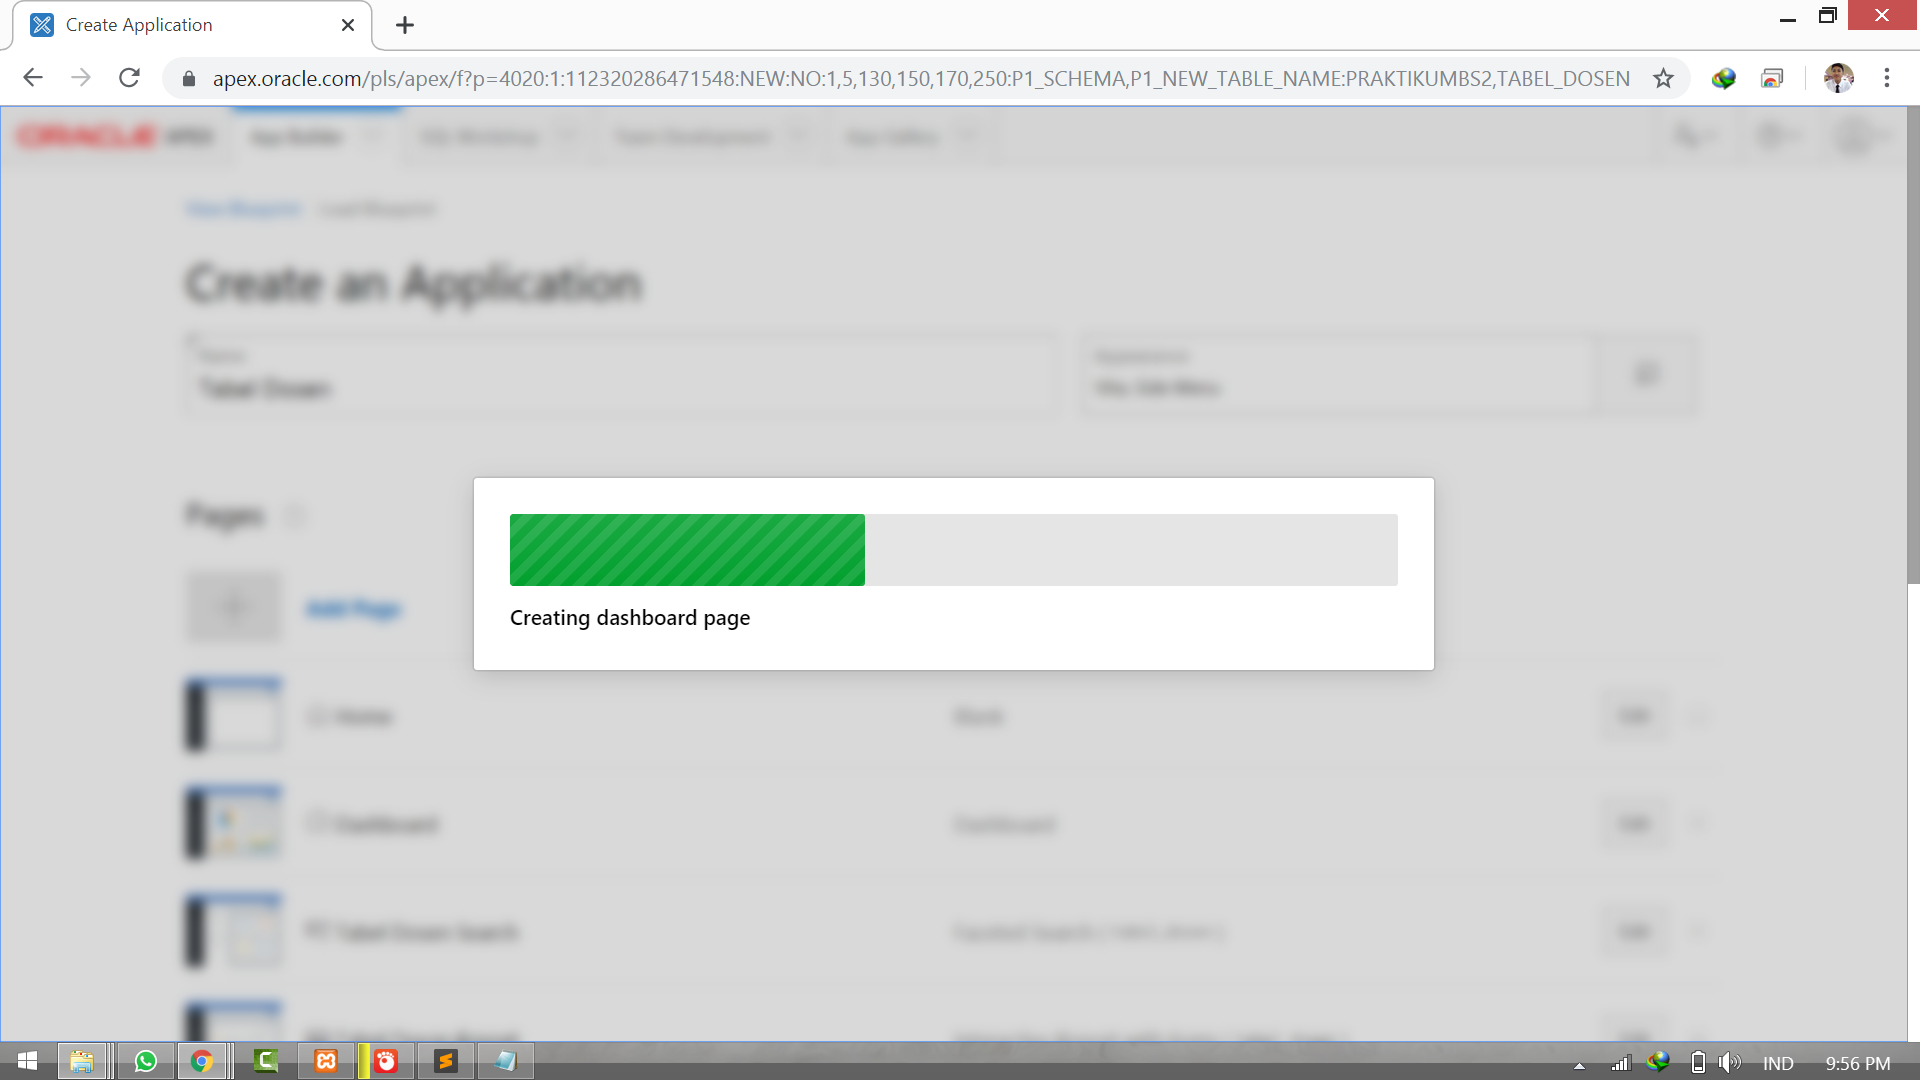
\includegraphics[scale=0.1]{img/11.png}}
        \centering
        \caption{}
		\label{langkah17}
	\end{figure}
	
\newpage
\item klik \textbf{app builder} lagi dan lakukan hal yang sama seperti yang dicontohkan sebelumnya
	\begin{figure}[h]
        \centerline{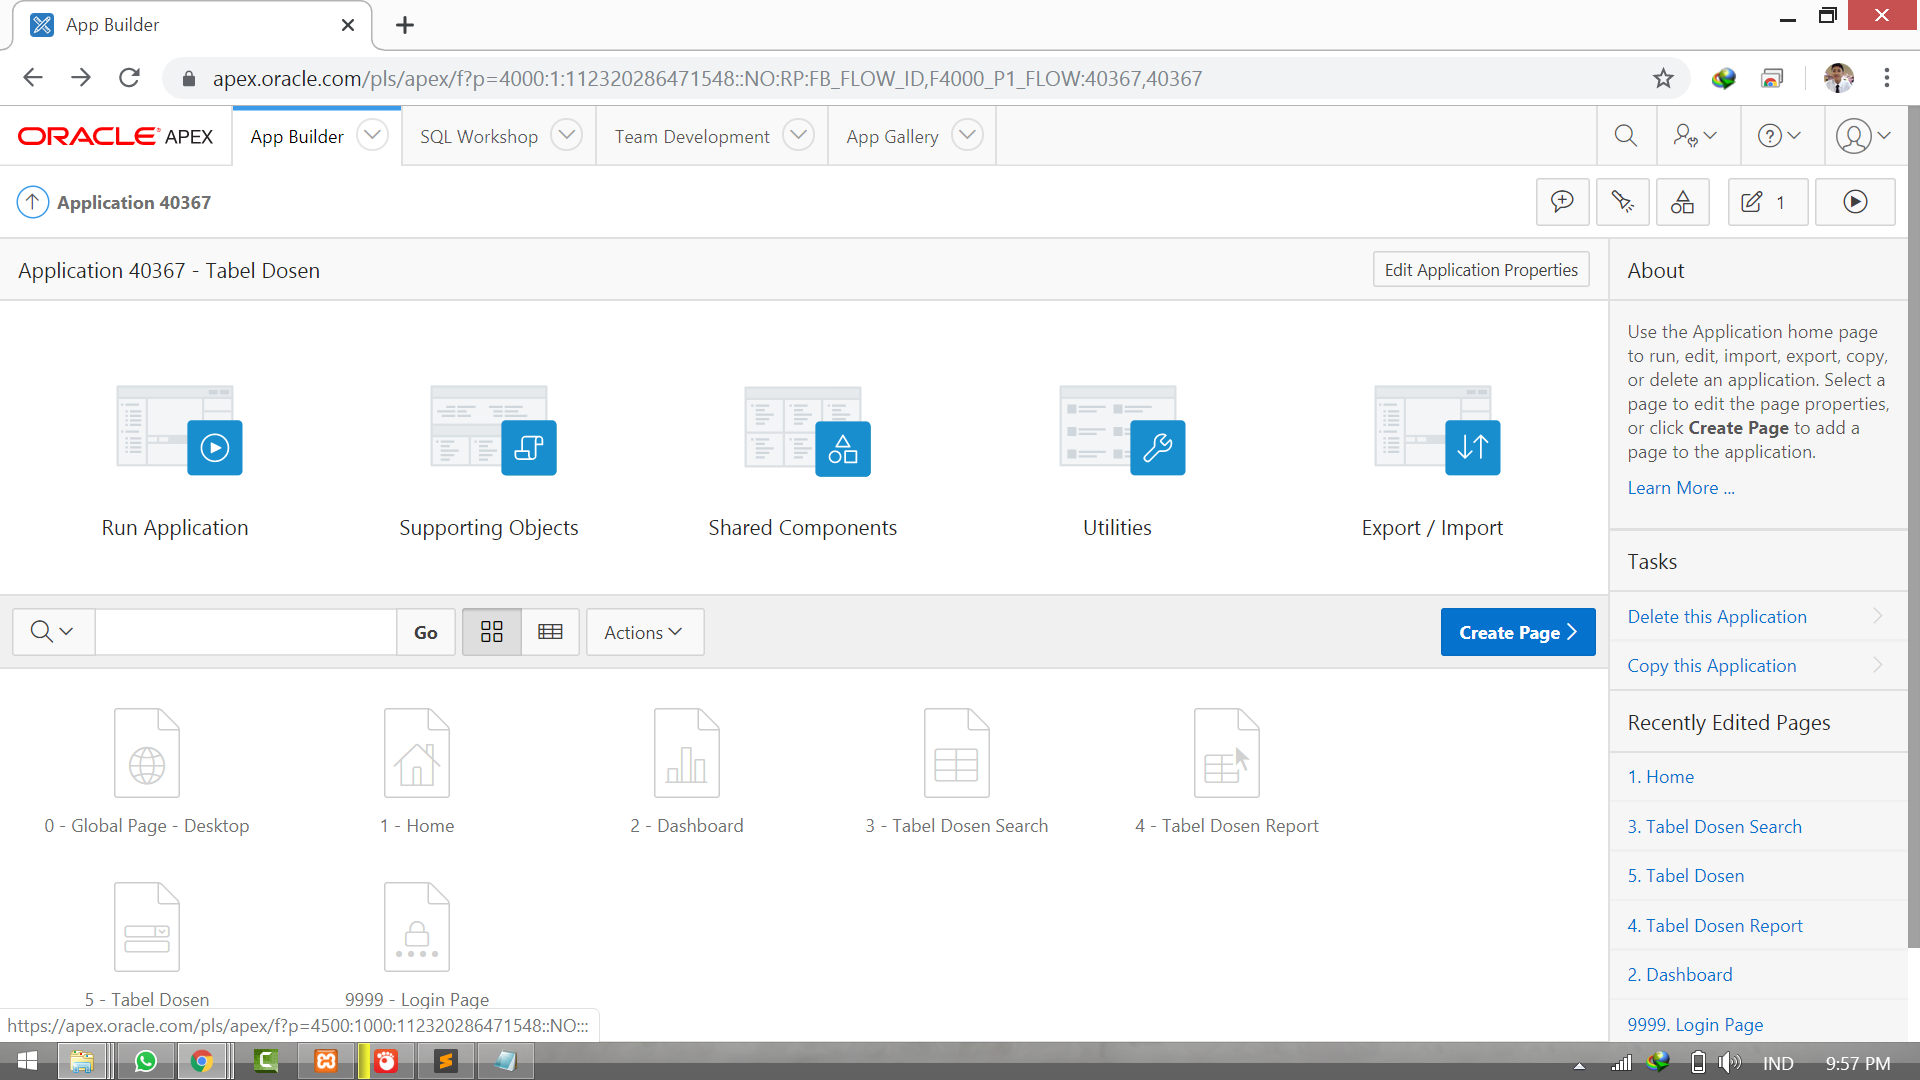
\includegraphics[scale=0.1]{img/12.png}}
        \centering
        \caption{}
		\label{langkah18}
	\end{figure}
	
\item pilih file tabel excel
	\begin{figure}[h]
        \centerline{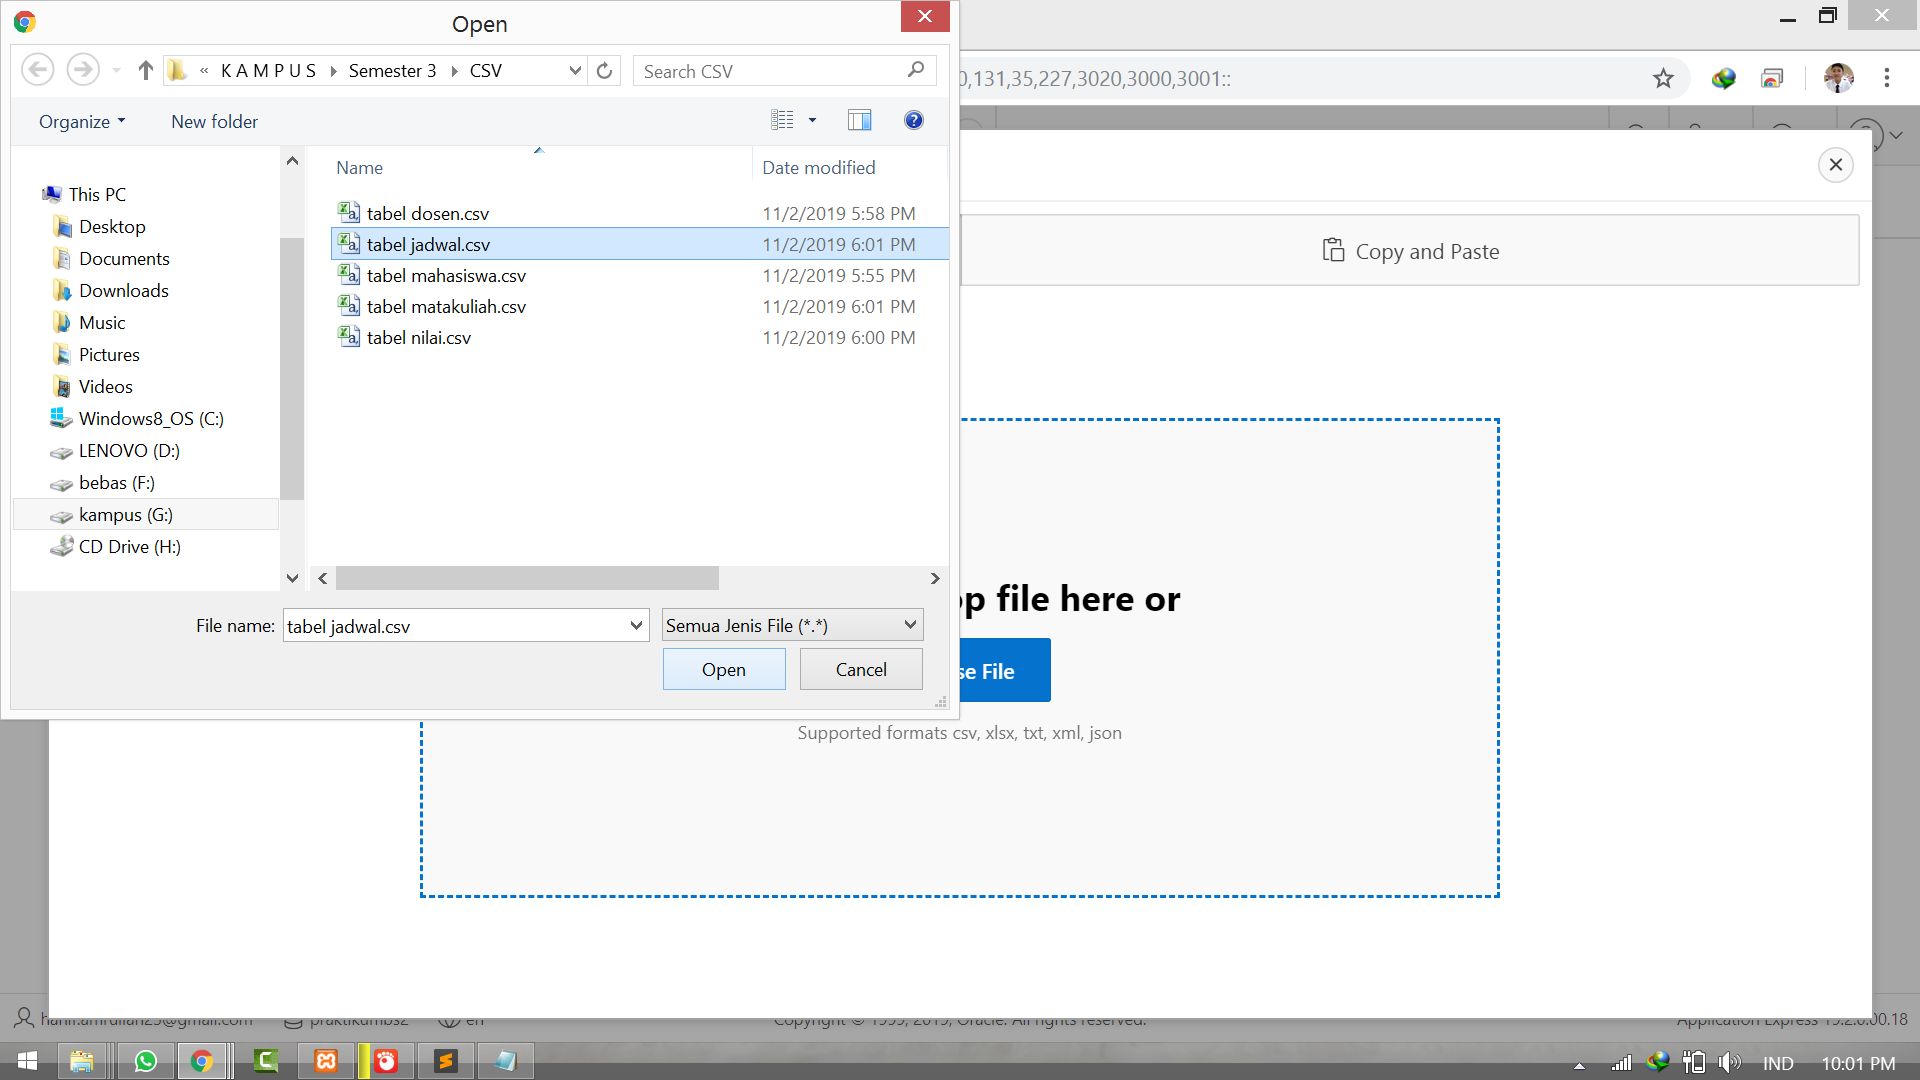
\includegraphics[scale=0.1]{img/13.png}}
        \centering
        \caption{}
		\label{langkah19}
	\end{figure}
	
\newpage
\item isi nama tabel di bagian \textbf{Table Name}, lalu klik \textbf{Load Data}
	\begin{figure}[h]
        \centerline{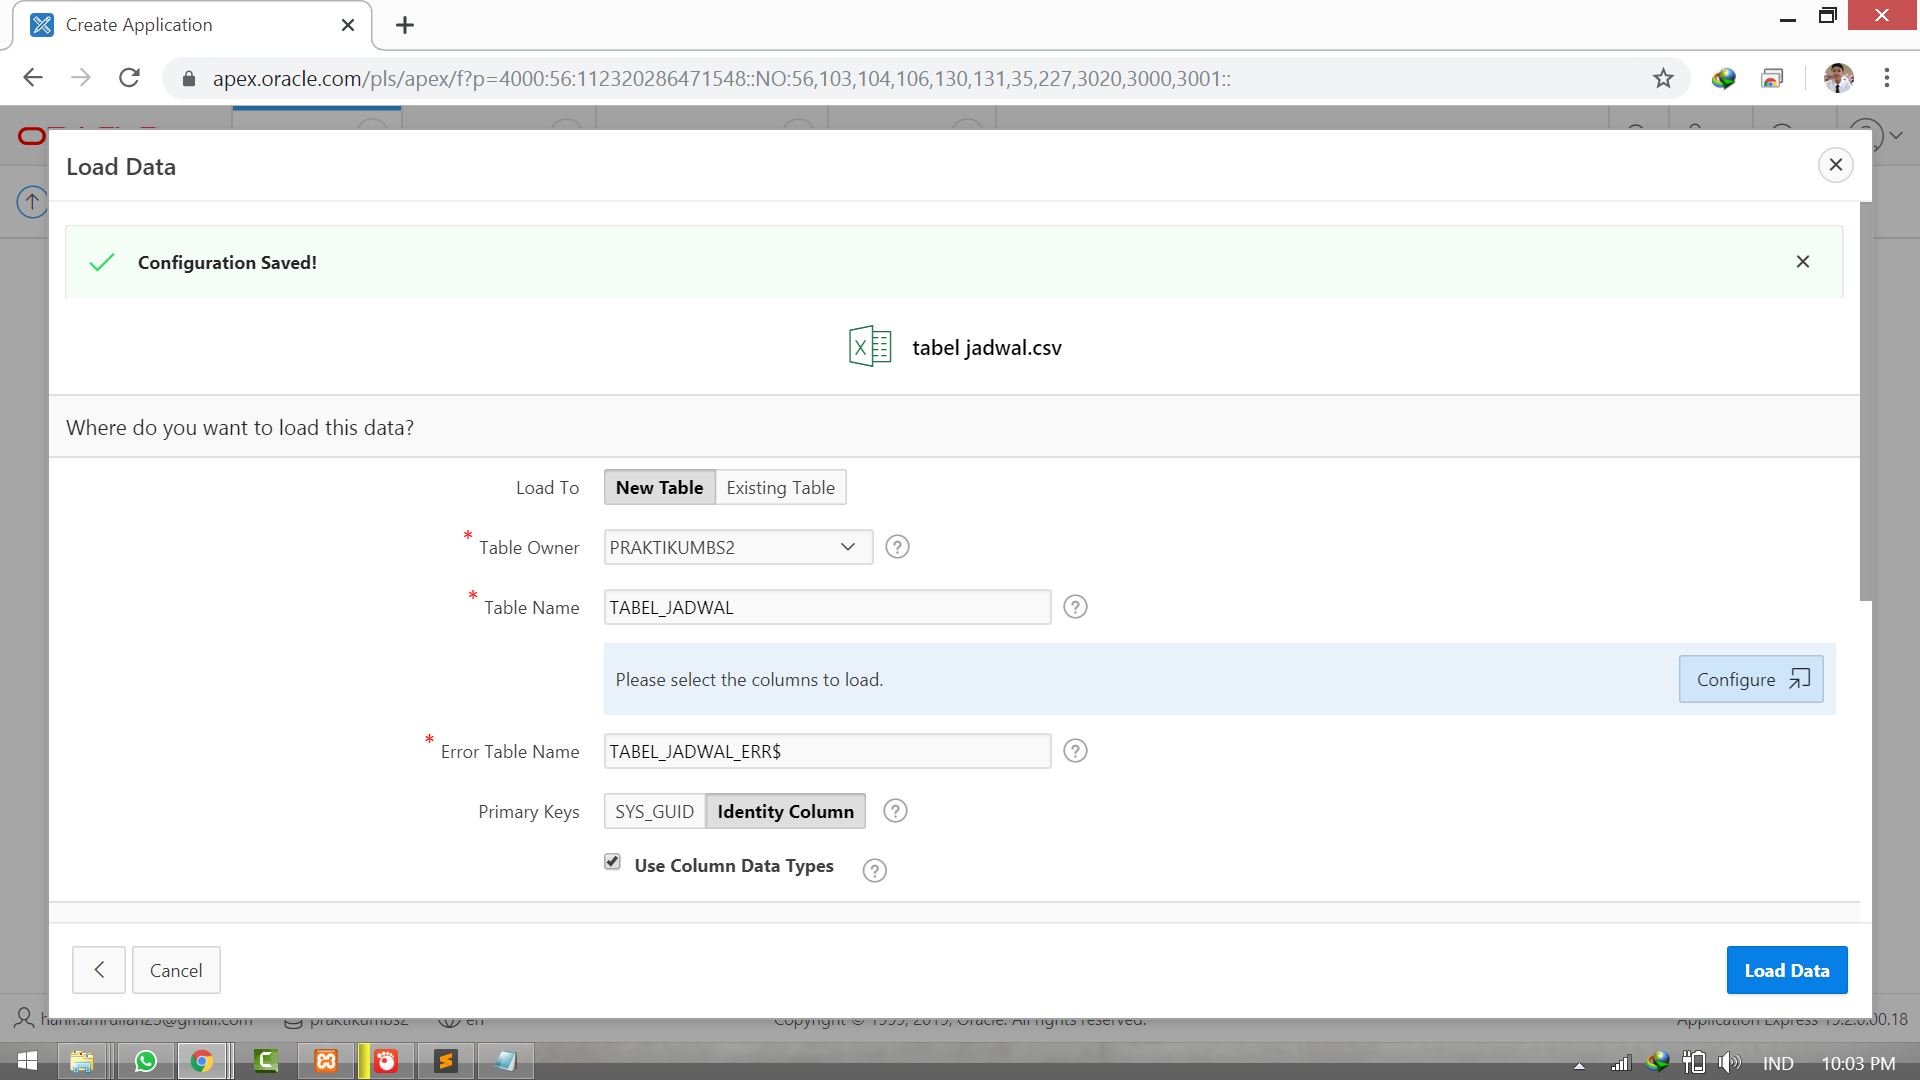
\includegraphics[scale=0.1]{img/14.png}}
        \centering
        \caption{}
		\label{langkah20}
	\end{figure}
	
\item klik \textbf{Create Application}
	\begin{figure}[h]
        \centerline{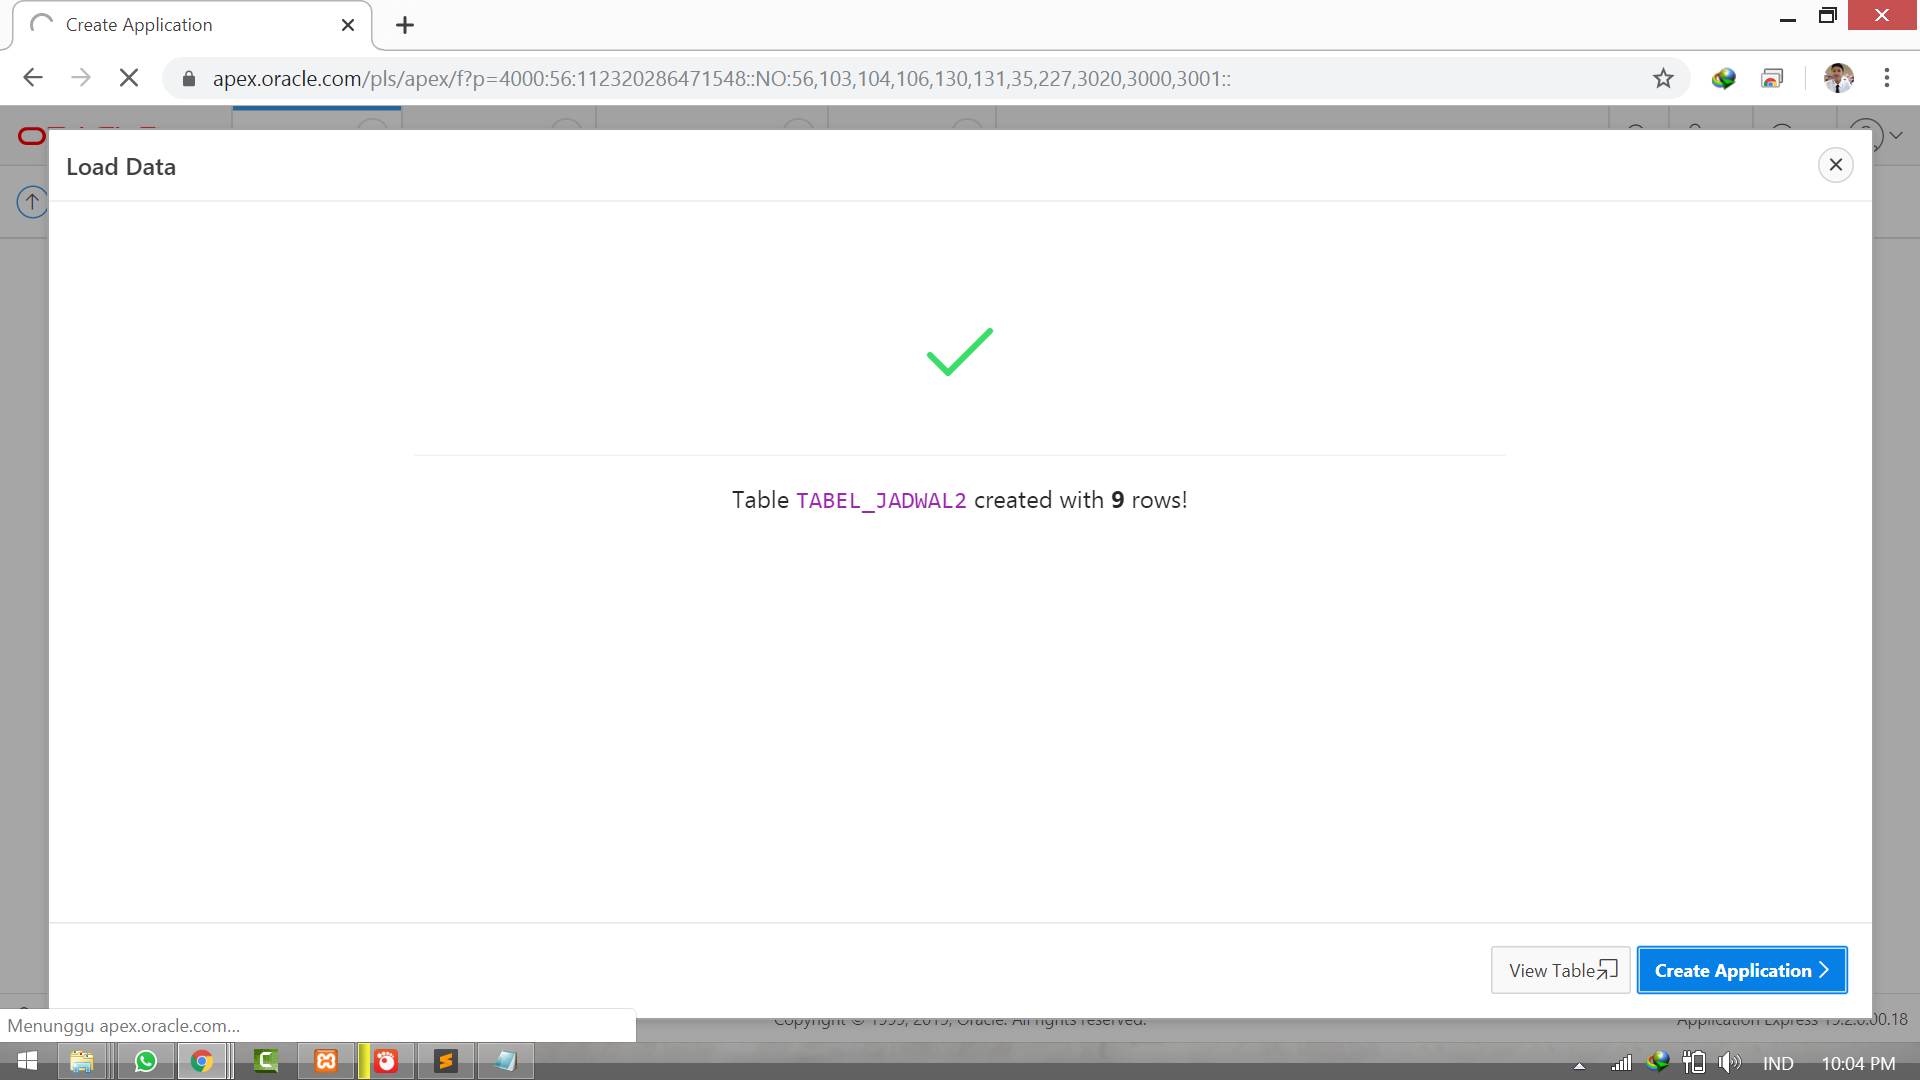
\includegraphics[scale=0.1]{img/15.png}}
        \centering
        \caption{}
		\label{langkah21}
	\end{figure}

\newpage
\item pilih file tabel excel
	\begin{figure}[h]
        \centerline{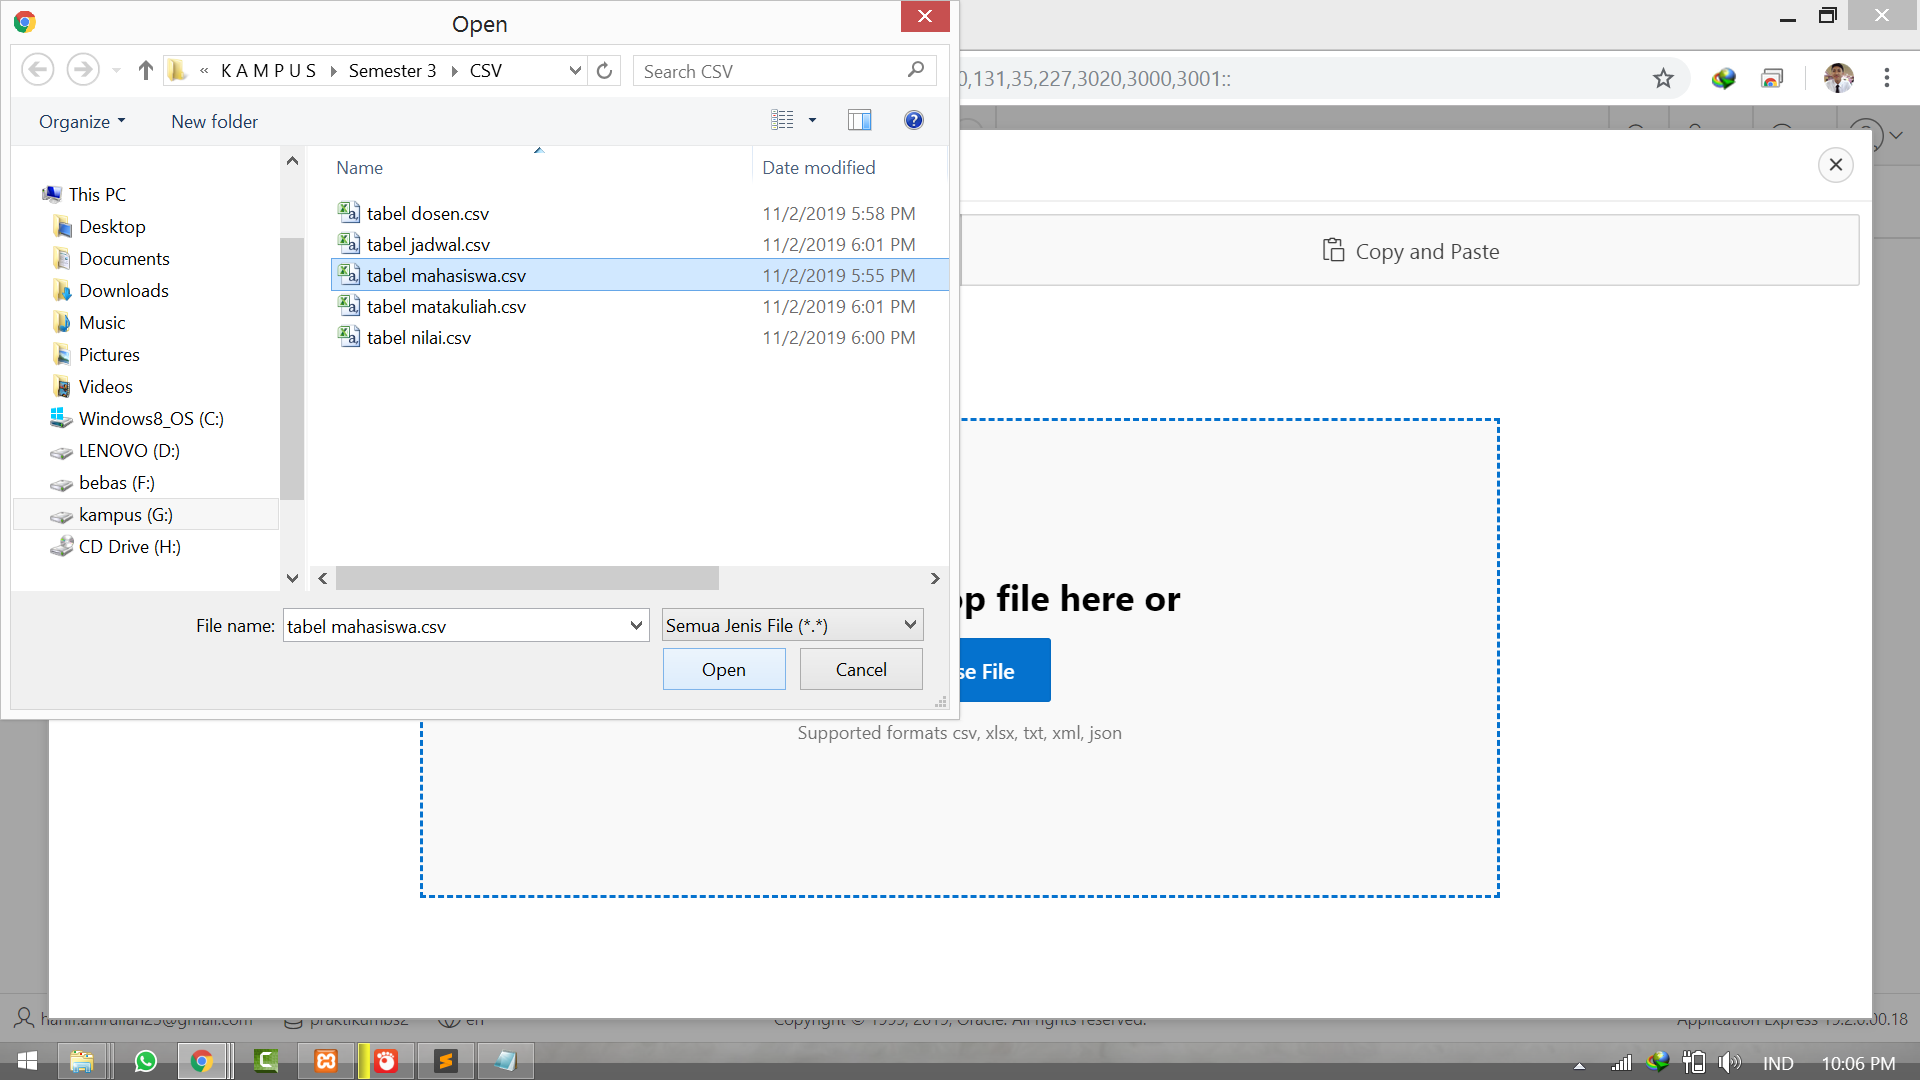
\includegraphics[scale=0.1]{img/16.png}}
        \centering
        \caption{}
		\label{langkah22}
	\end{figure}
	
\item isi nama tabel di bagian \textbf{Table Name}, lalu klik \textbf{Load Data}
	\begin{figure}[h]
        \centerline{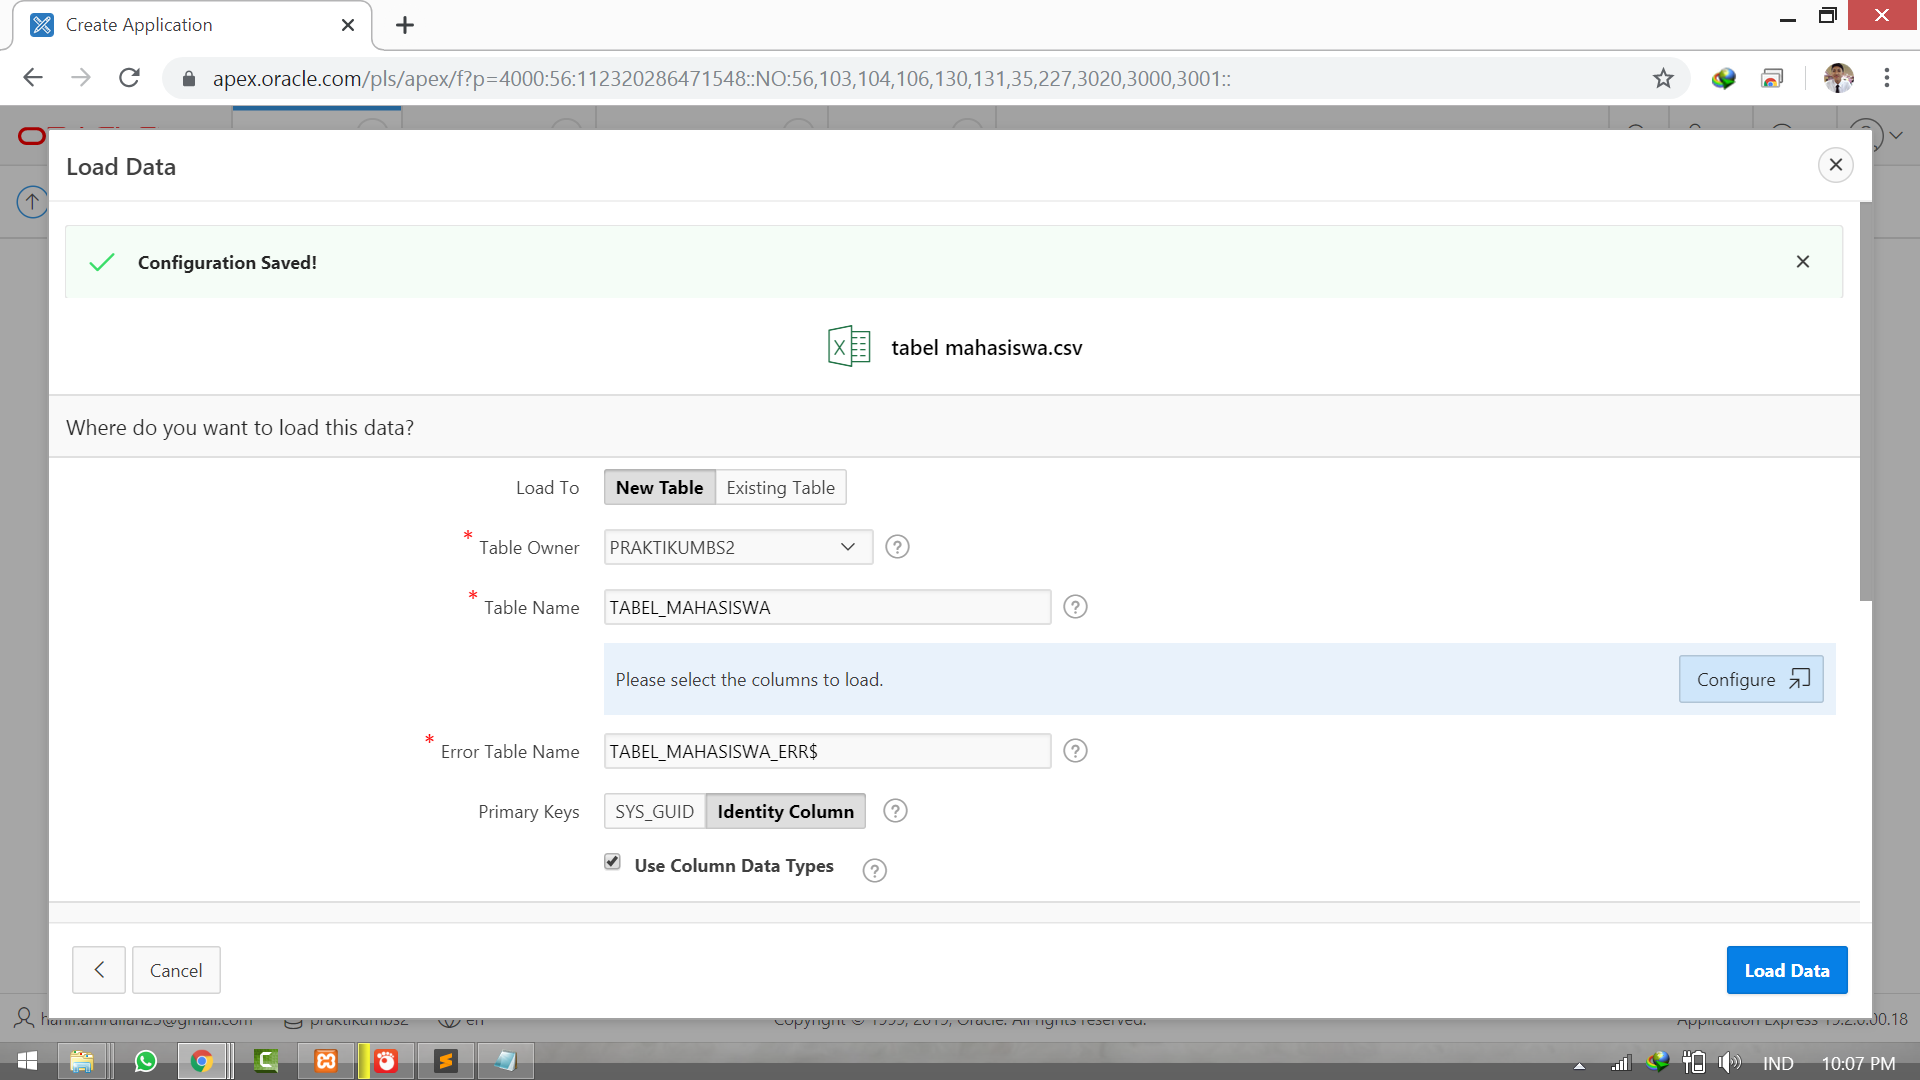
\includegraphics[scale=0.1]{img/17.png}}
        \centering
        \caption{}
		\label{langkah23}
	\end{figure}
	
\newpage
\item klik \textbf{Create Application}
	\begin{figure}[h]
        \centerline{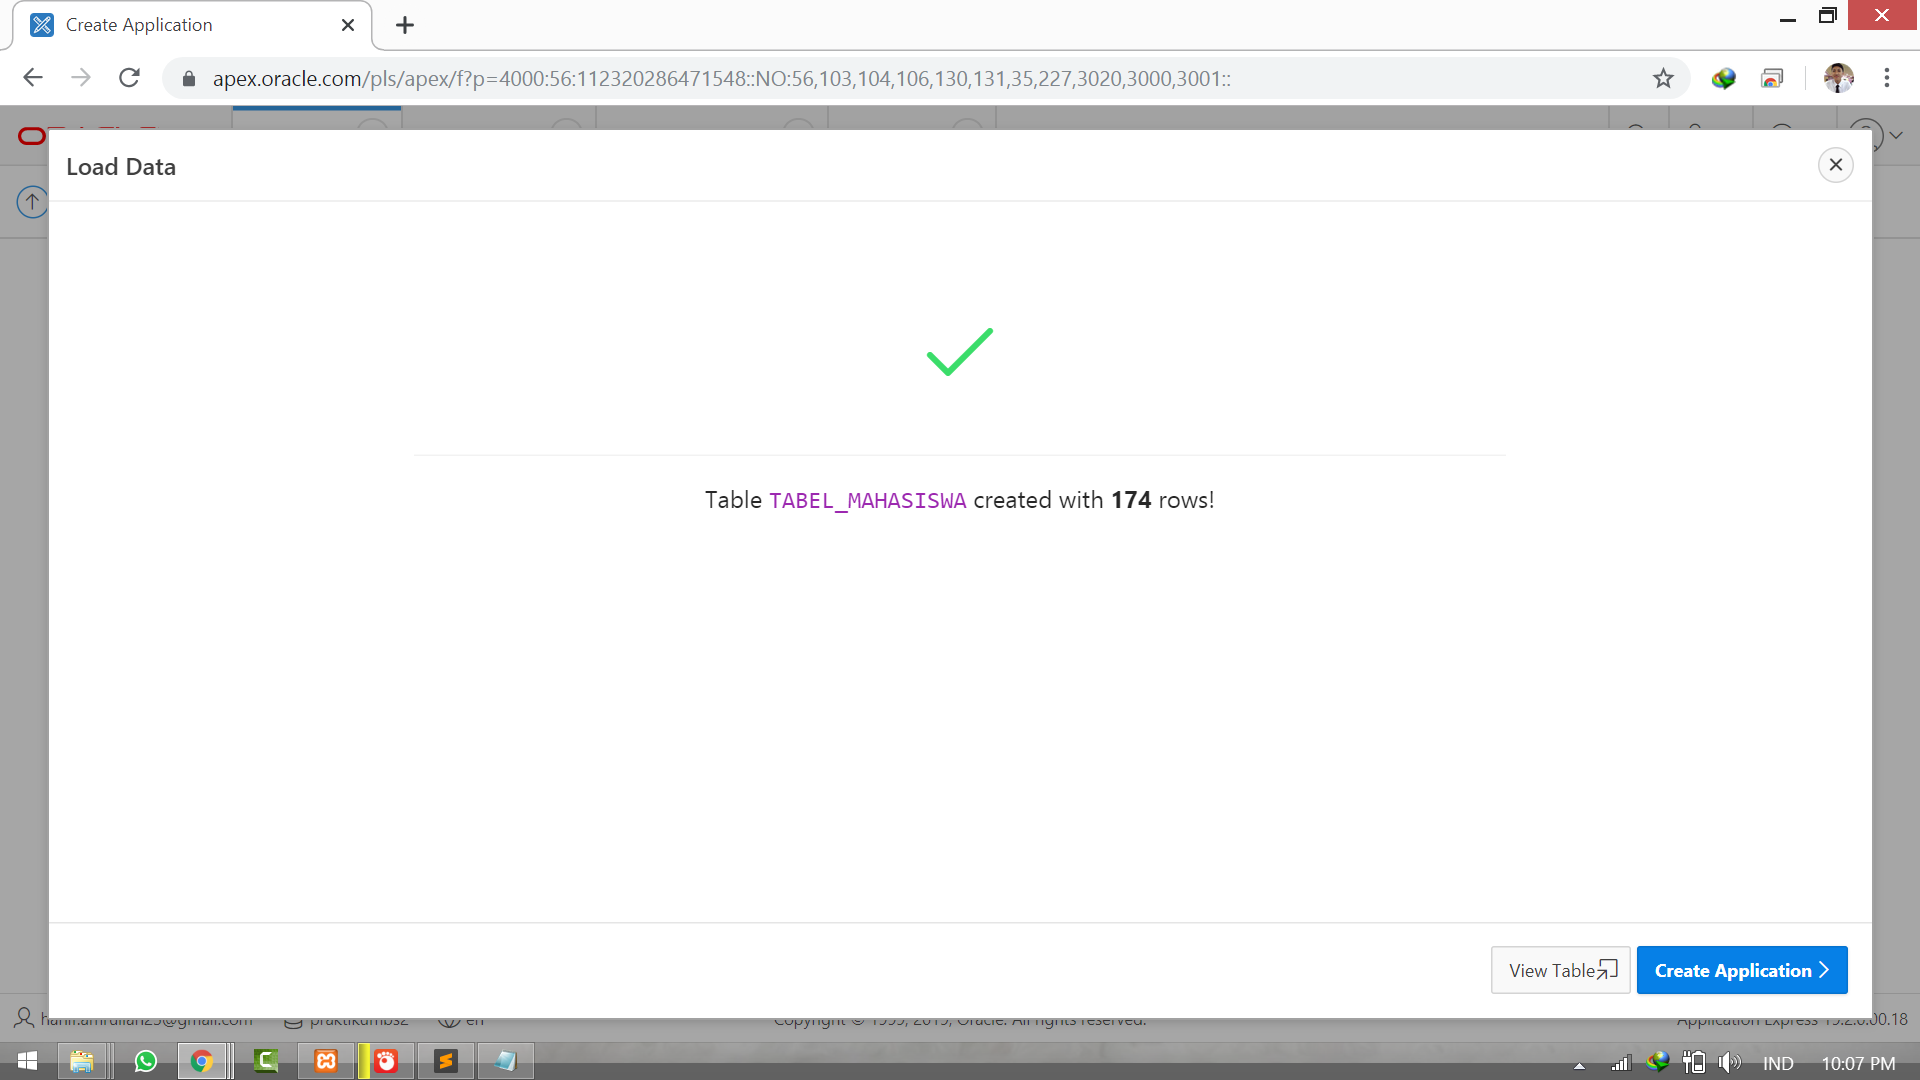
\includegraphics[scale=0.1]{img/18.png}}
        \centering
        \caption{}
		\label{langkah24}
	\end{figure}
	
\item pilih file tabel excel
	\begin{figure}[h]
        \centerline{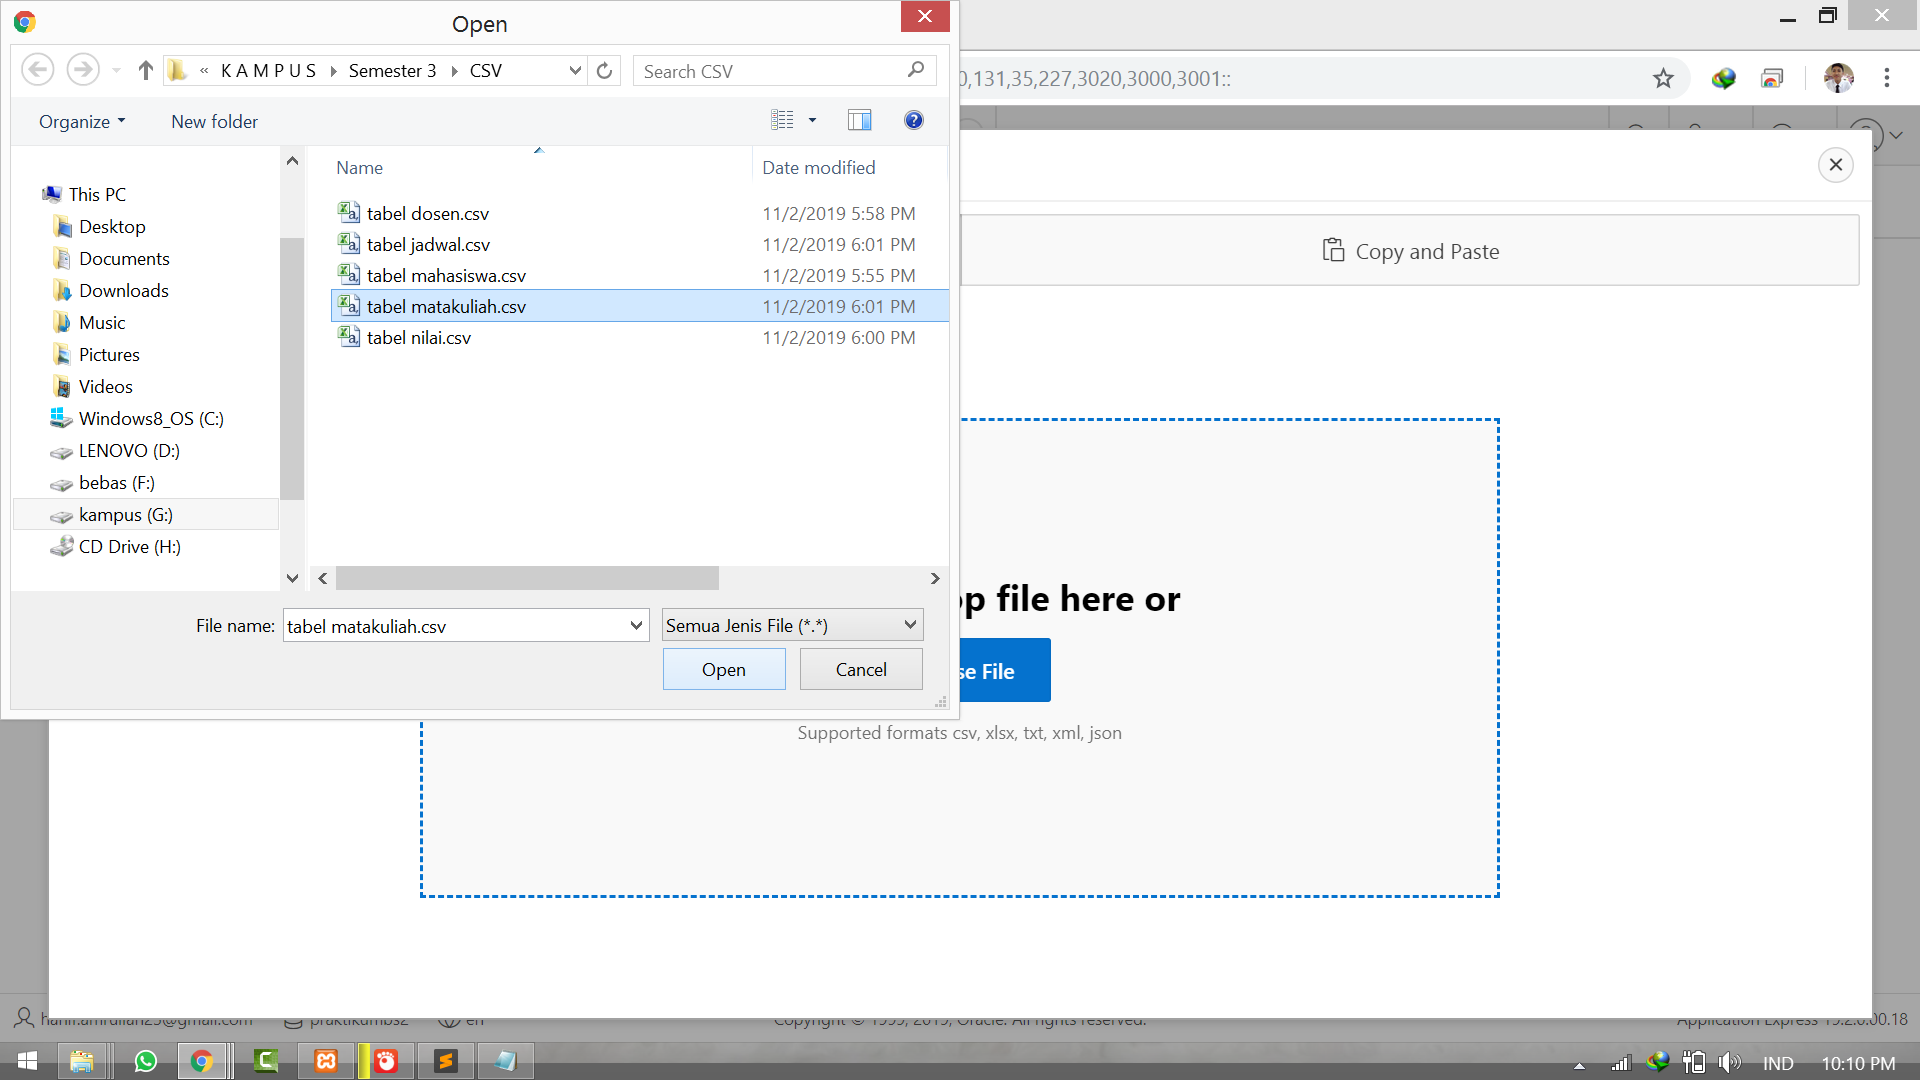
\includegraphics[scale=0.1]{img/19.png}}
        \centering
        \caption{}
		\label{langkah25}
	\end{figure}
	
\newpage
\item isi nama tabel di bagian \textbf{Table Name}, lalu klik \textbf{Load Data}
	\begin{figure}[h]
        \centerline{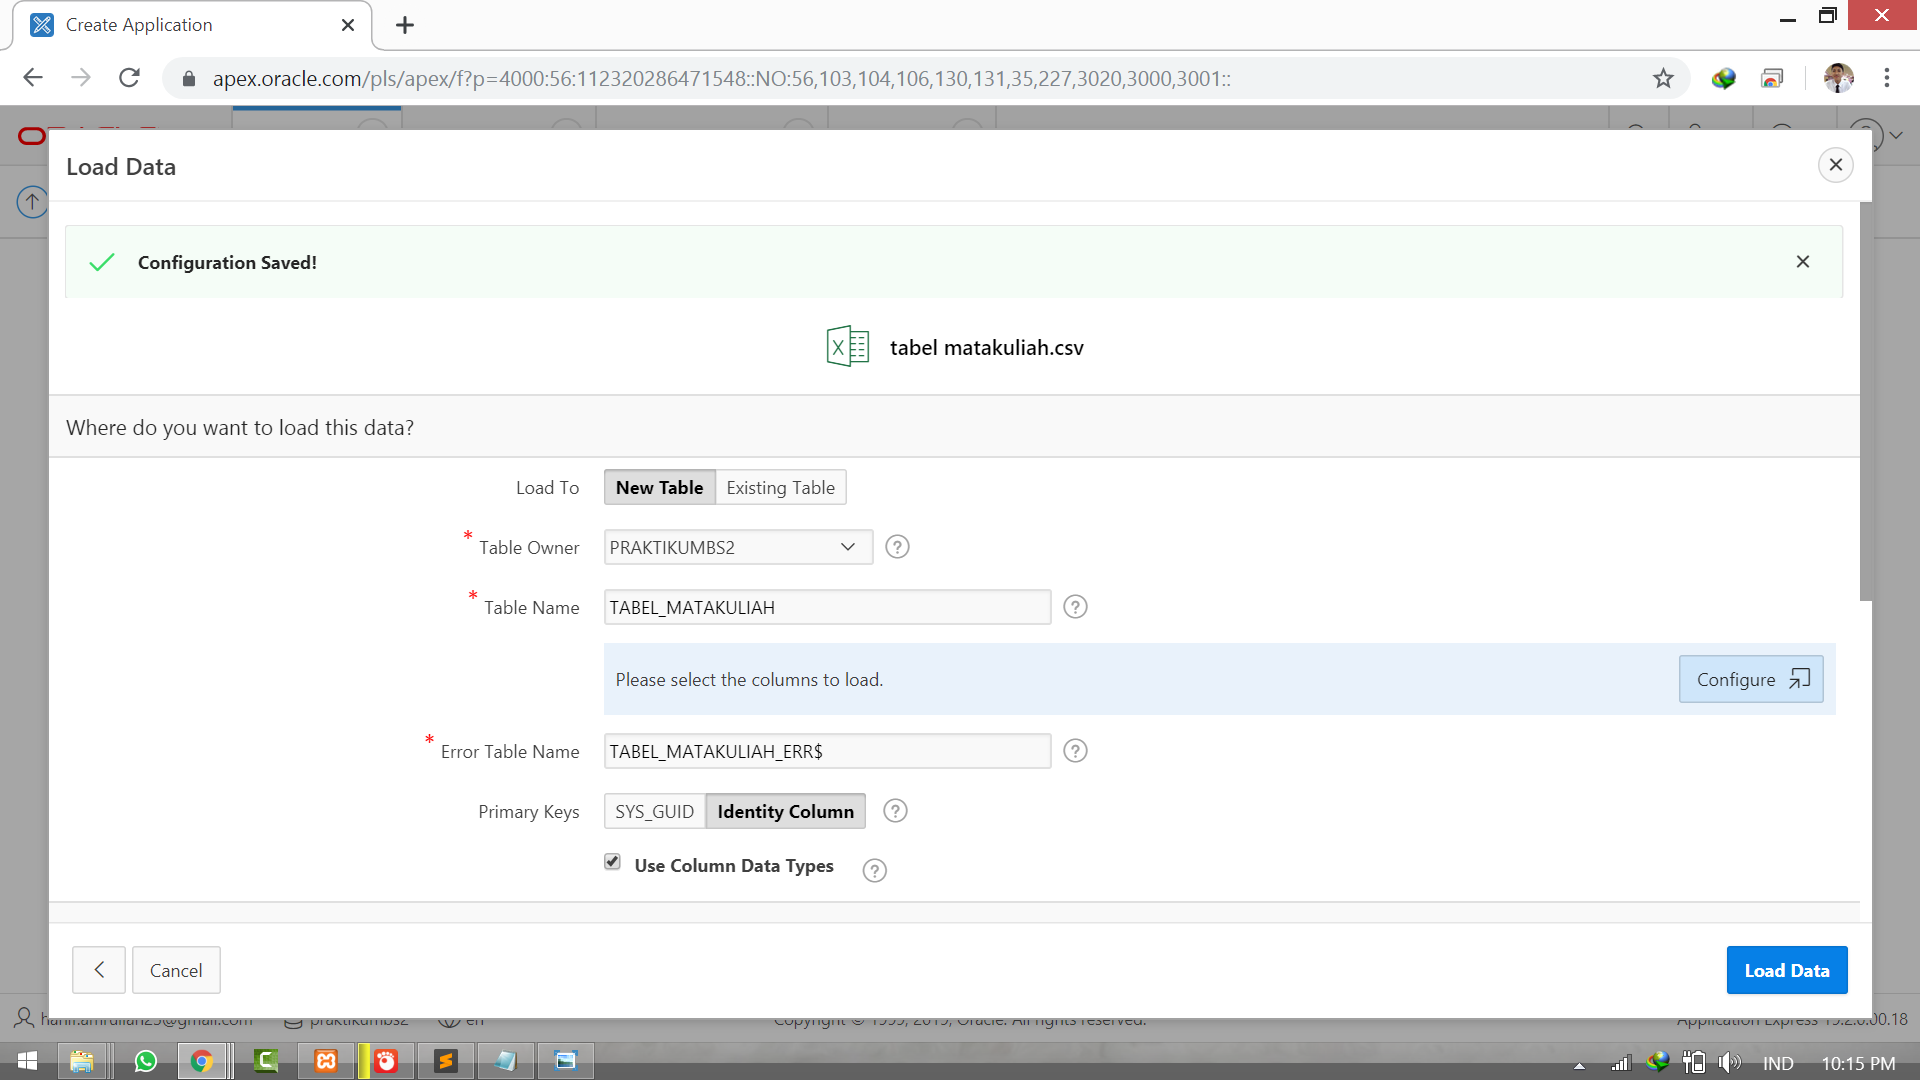
\includegraphics[scale=0.1]{img/20.png}}
        \centering
        \caption{}
		\label{langkah26}
	\end{figure}
	
\item klik \textbf{Create Application}
	\begin{figure}[h]
        \centerline{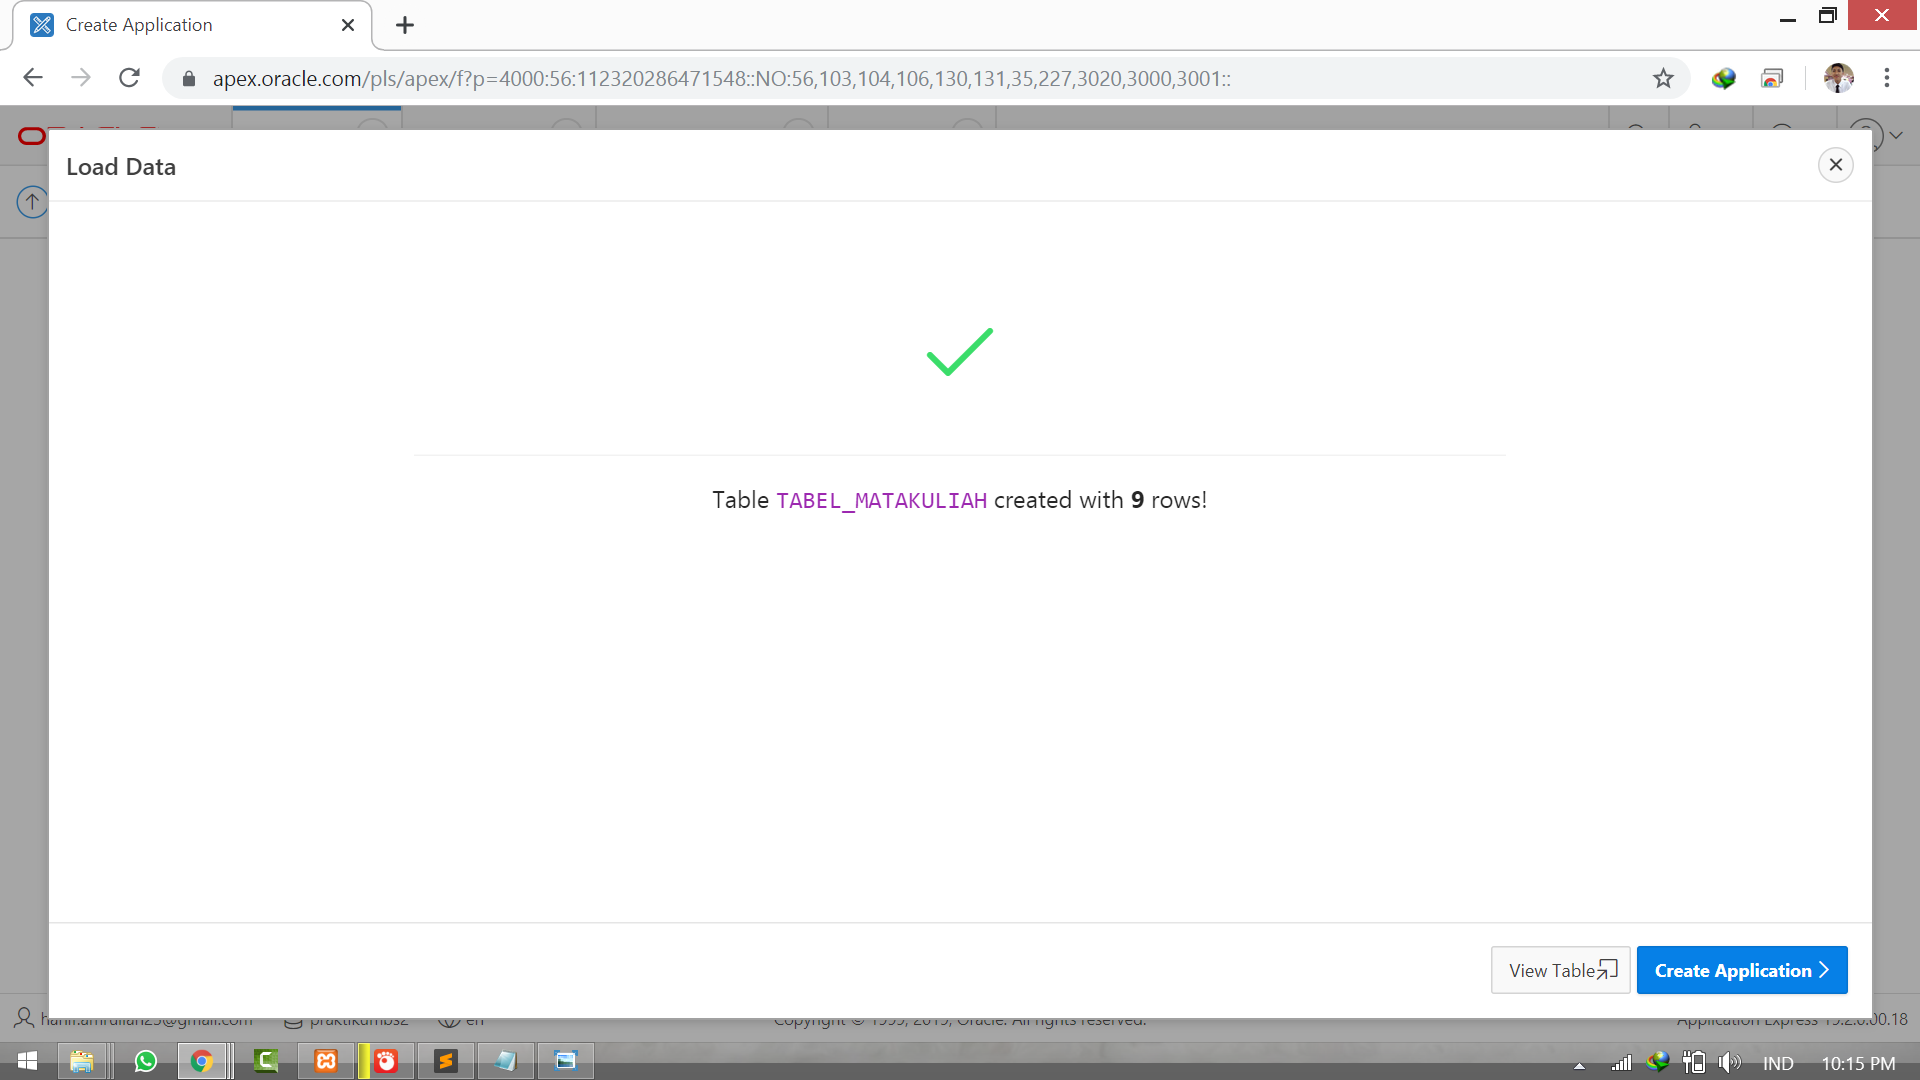
\includegraphics[scale=0.1]{img/21.png}}
        \centering
        \caption{}
		\label{langkah27}
	\end{figure}
	
\newpage
\item pilih file tabel excel dan seterusnya, seperti contoh langkah-langkah sebelumnya yang sudah di jelaskan
	\begin{figure}[h]
        \centerline{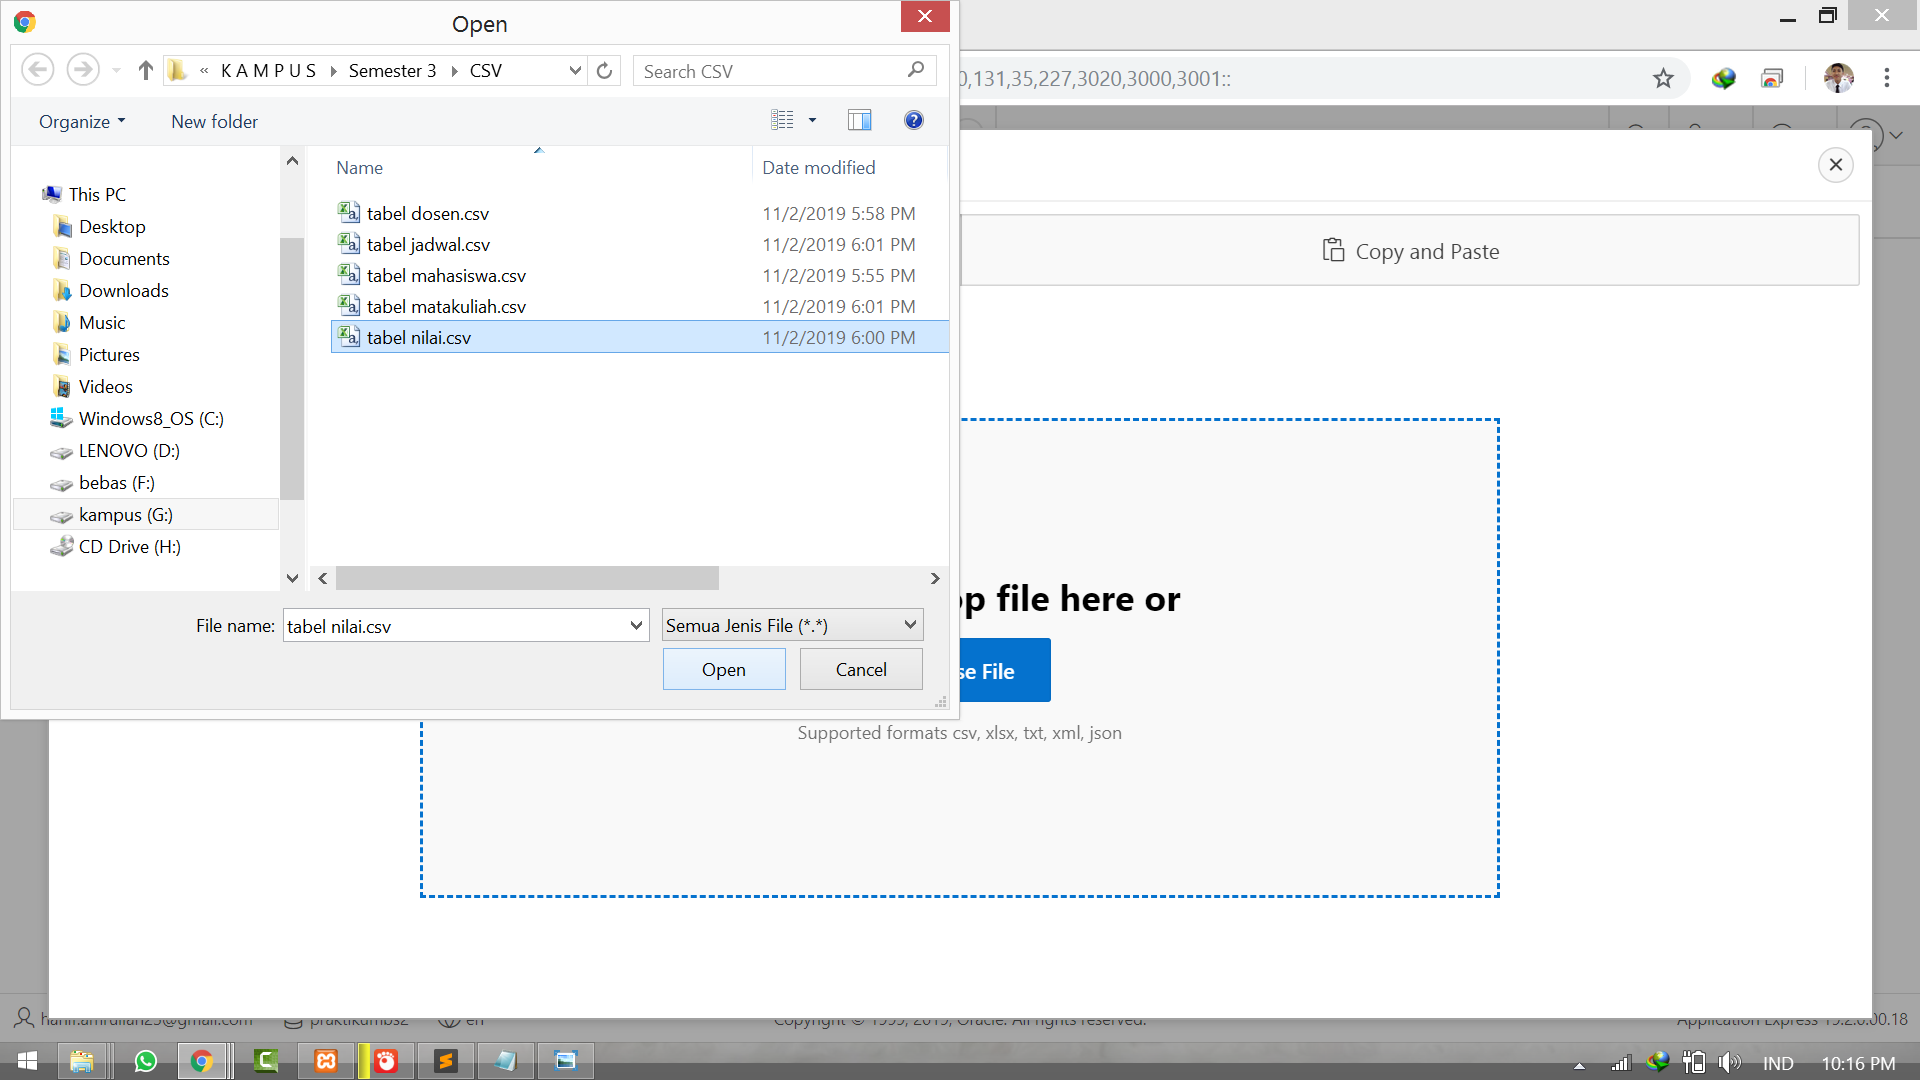
\includegraphics[scale=0.1]{img/22.png}}
        \centering
        \caption{}
		\label{langkah22}
	\end{figure}
	
\item
setelah selesai mengupload data yang dibutuhkan, selanjutnya klik tabel \textbf{SQL Workshop}, klik \textbf{Object Browser}
	\begin{figure}[h]
        \centerline{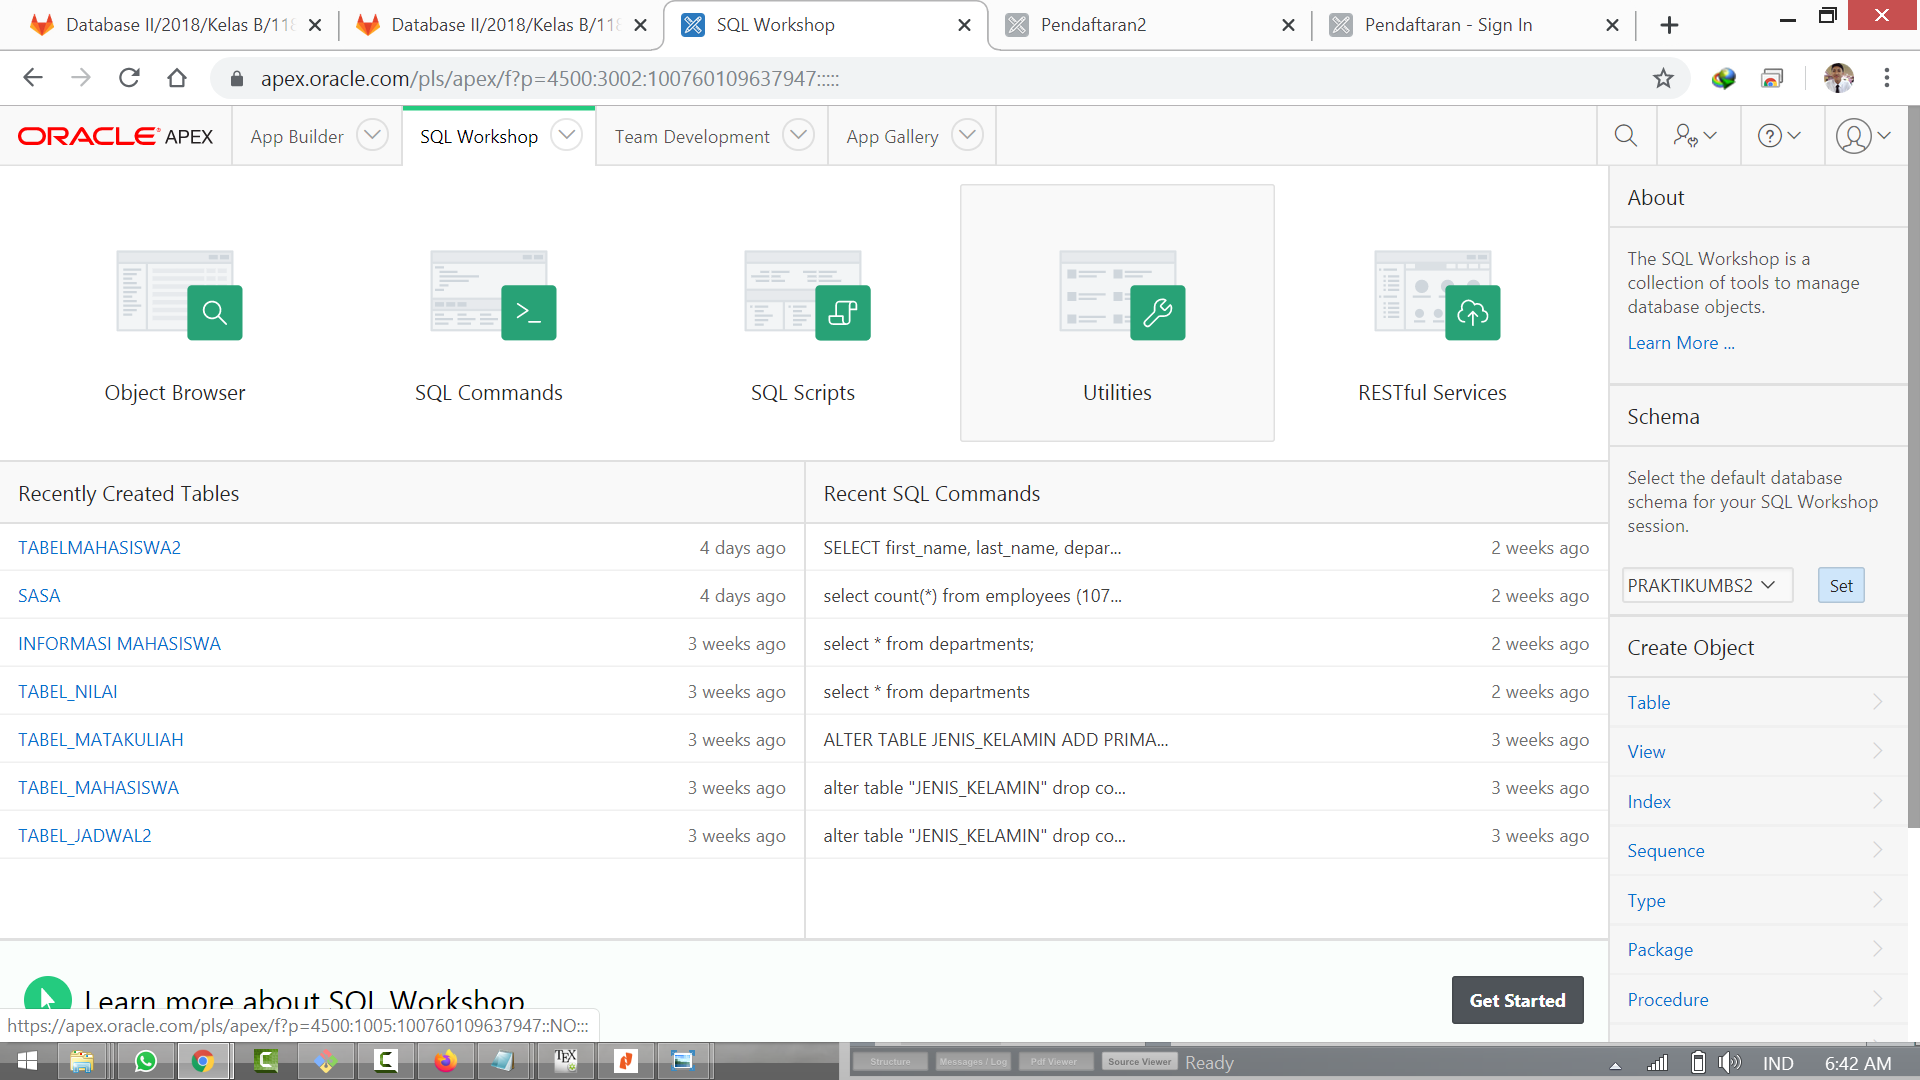
\includegraphics[scale=0.1]{img/b1.png}}
        \centering
        \caption{}
		\label{langkah23}
	\end{figure}
	
\newpage
klik tabel yang sudah kita upload lalu \textit{Drop Colomn} tiap masing-masing table untuk meng\textbf{remove colomn "ID"}
	\begin{figure}[h]
        \centerline{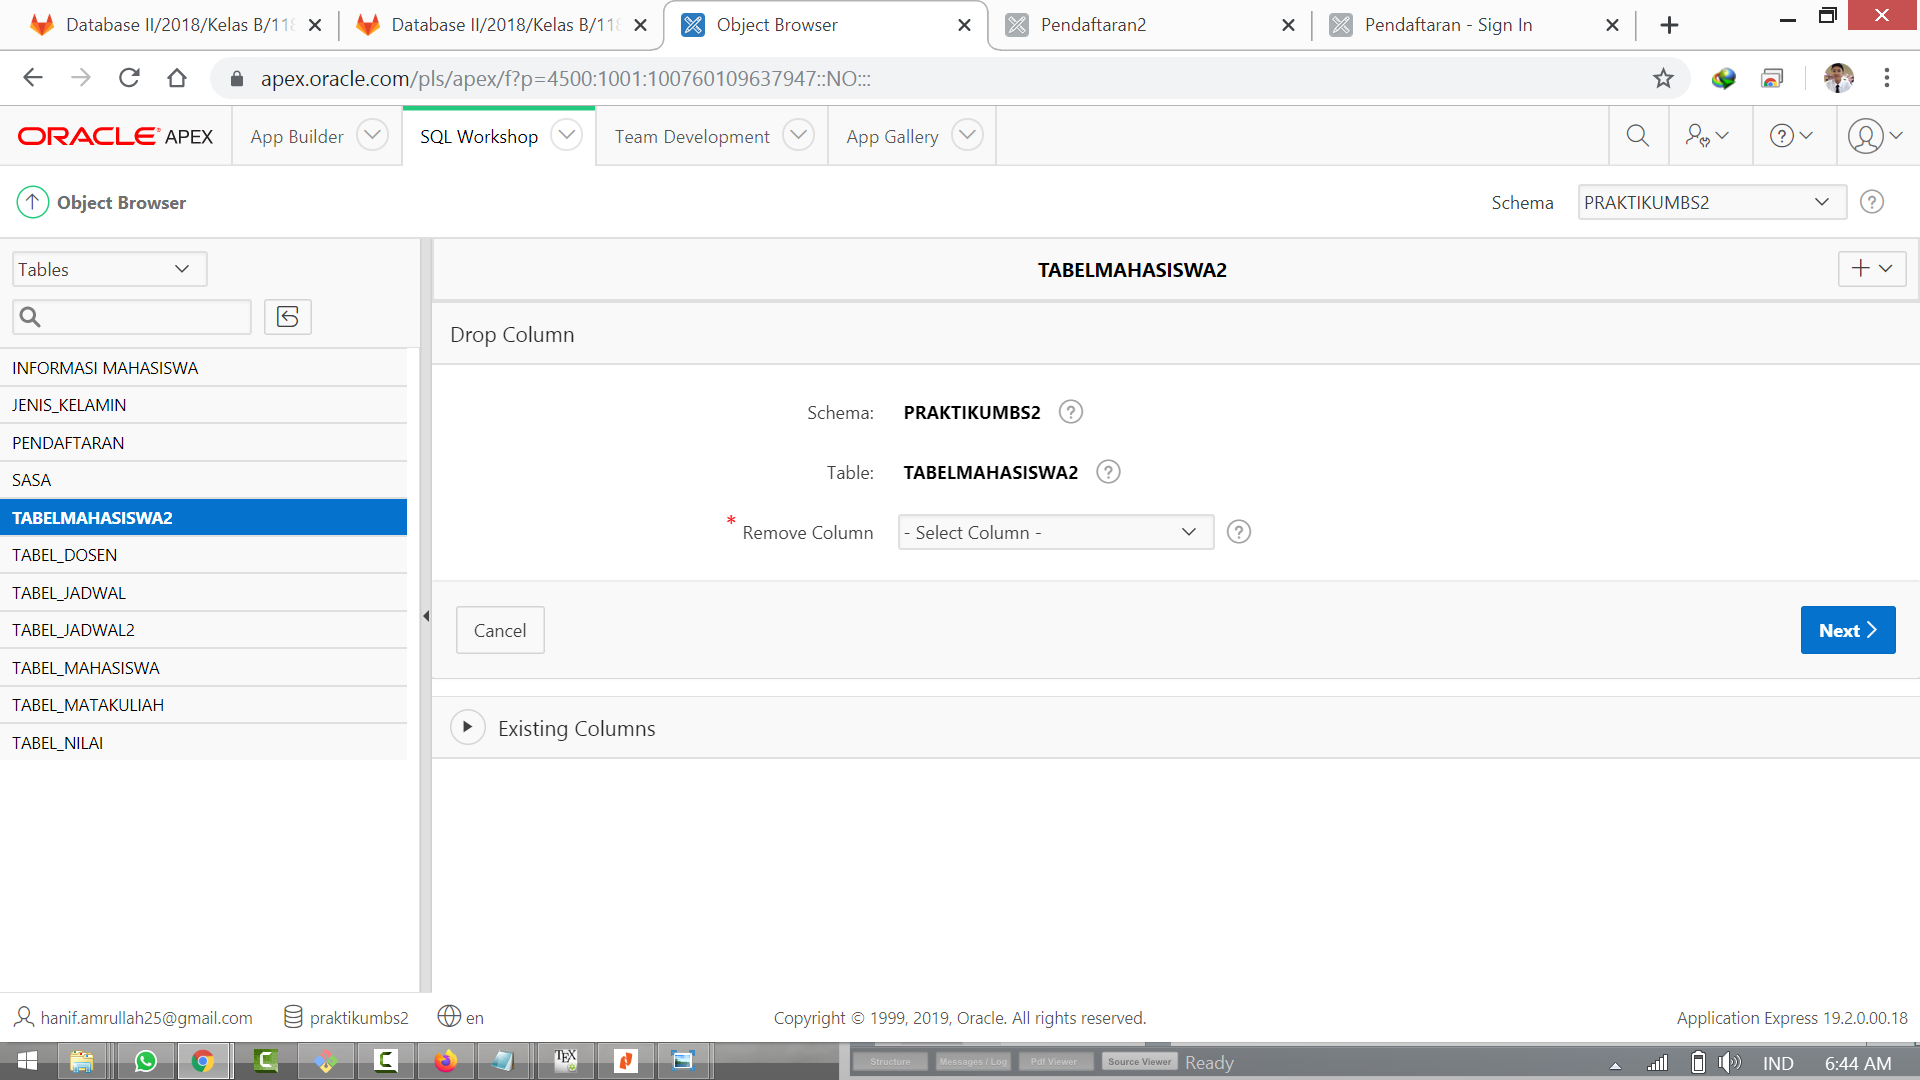
\includegraphics[scale=0.1]{img/b2.png}}
        \centering
        \caption{}
		\label{langkah24}
	\end{figure}
	
\item
setelah semua tabel sudah kita drop colom langkah selanjutnya ialah buka \textbf{SQL Command} disini kita akan melakukan perintah menentukan primary key untuk mengambil \textit{unique} yang nanti tidak dapat disamakan

\item
setelah  selesai melakukan perintah primary key, selanjutnya ialah menentukan perintah \textit{Foreign Key} 

\item 
jika data telah selesao kita atur perintah \textit{primary key dan foreign key}, langkah selanjutnya membuat aplikasi

\item klik \textbf{App Build}
\item klik \textbf{create}, lalu pilih \textbf{New Application}.
	\begin{figure}[h]
        \centerline{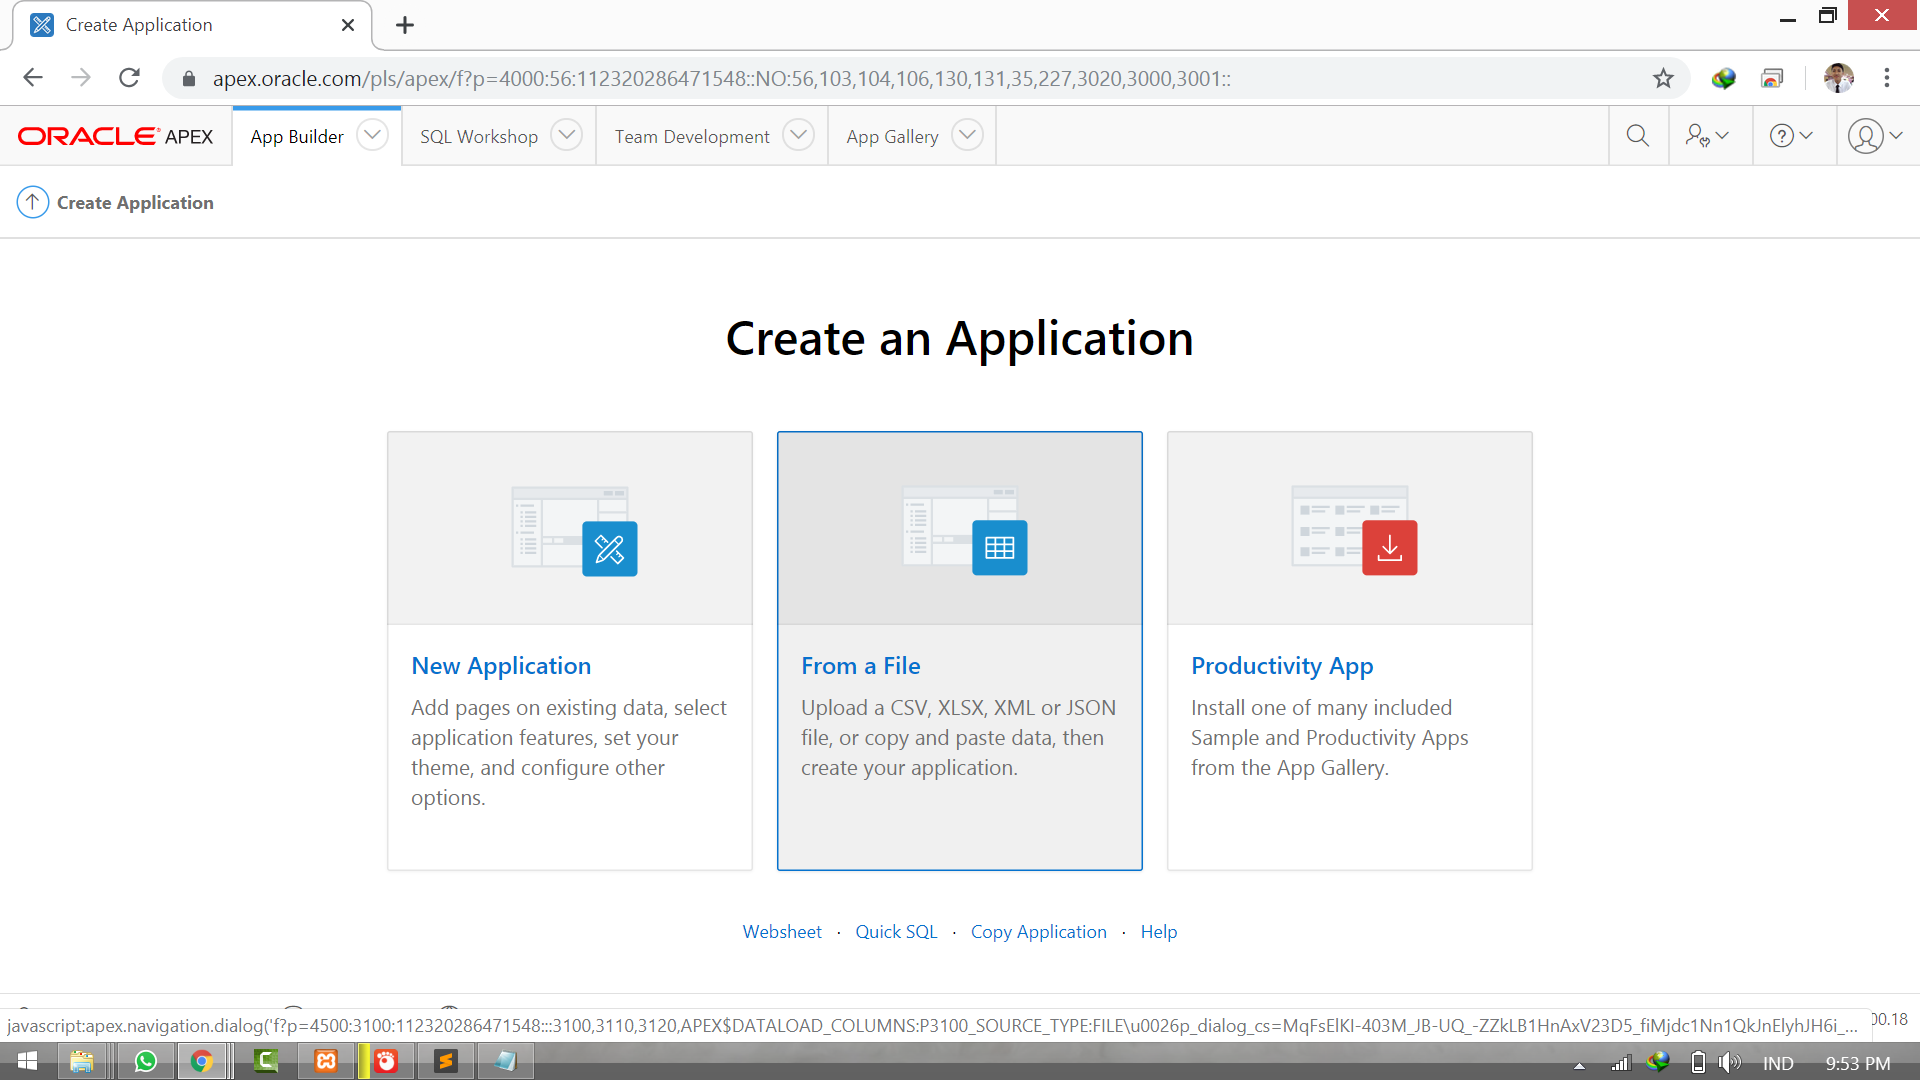
\includegraphics[scale=0.1]{img/4.png}}
        \centering
        \caption{}
		\label{langkah25}
	\end{figure}

\newpage
\item Tambahkan saja tabel yang kita perlu, lalu klik \textbf{Create Application}
	\begin{figure}[h]
        \centerline{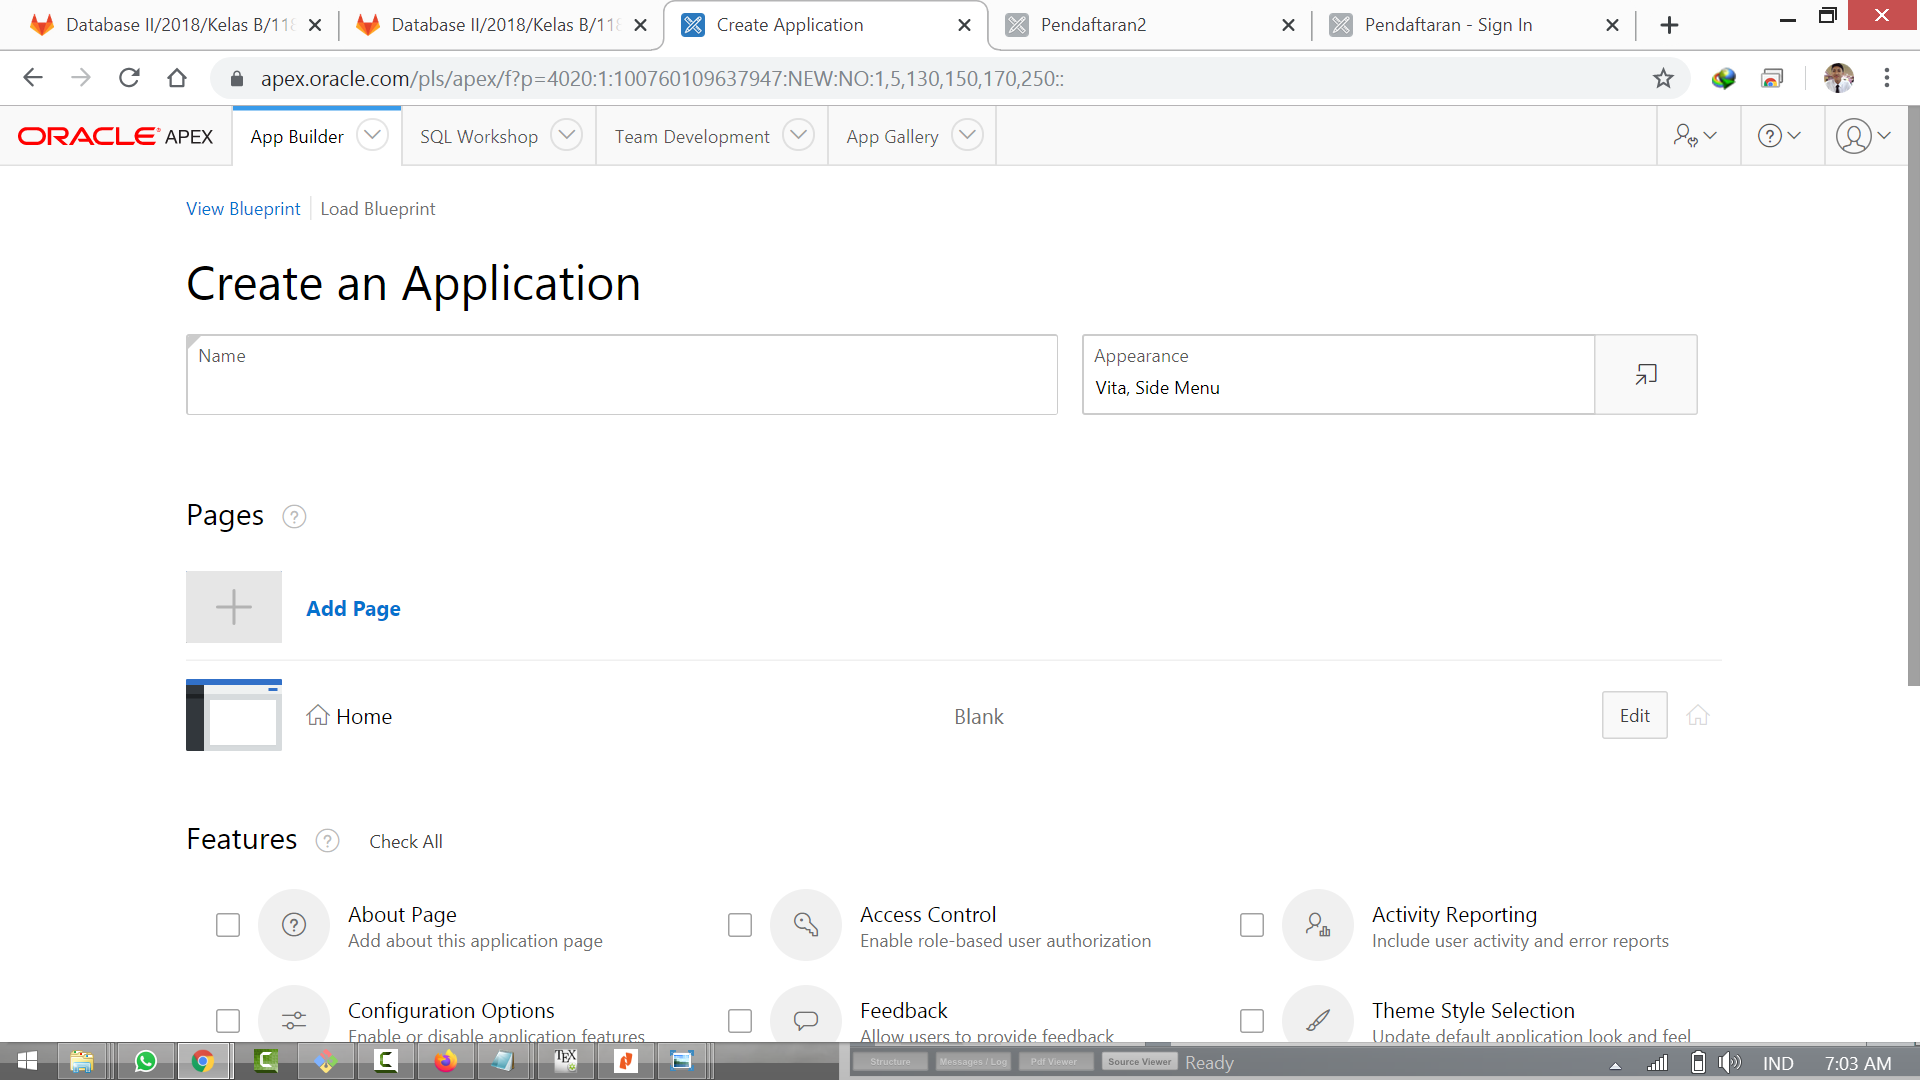
\includegraphics[scale=0.1]{img/b3.png}}
        \centering
        \caption{}
		\label{langkah26}
	\end{figure}

\item
setelah selesai maka coba \textit{run}, jika berhasil akan tampil seperti ini
	\begin{figure}[h]
        \centerline{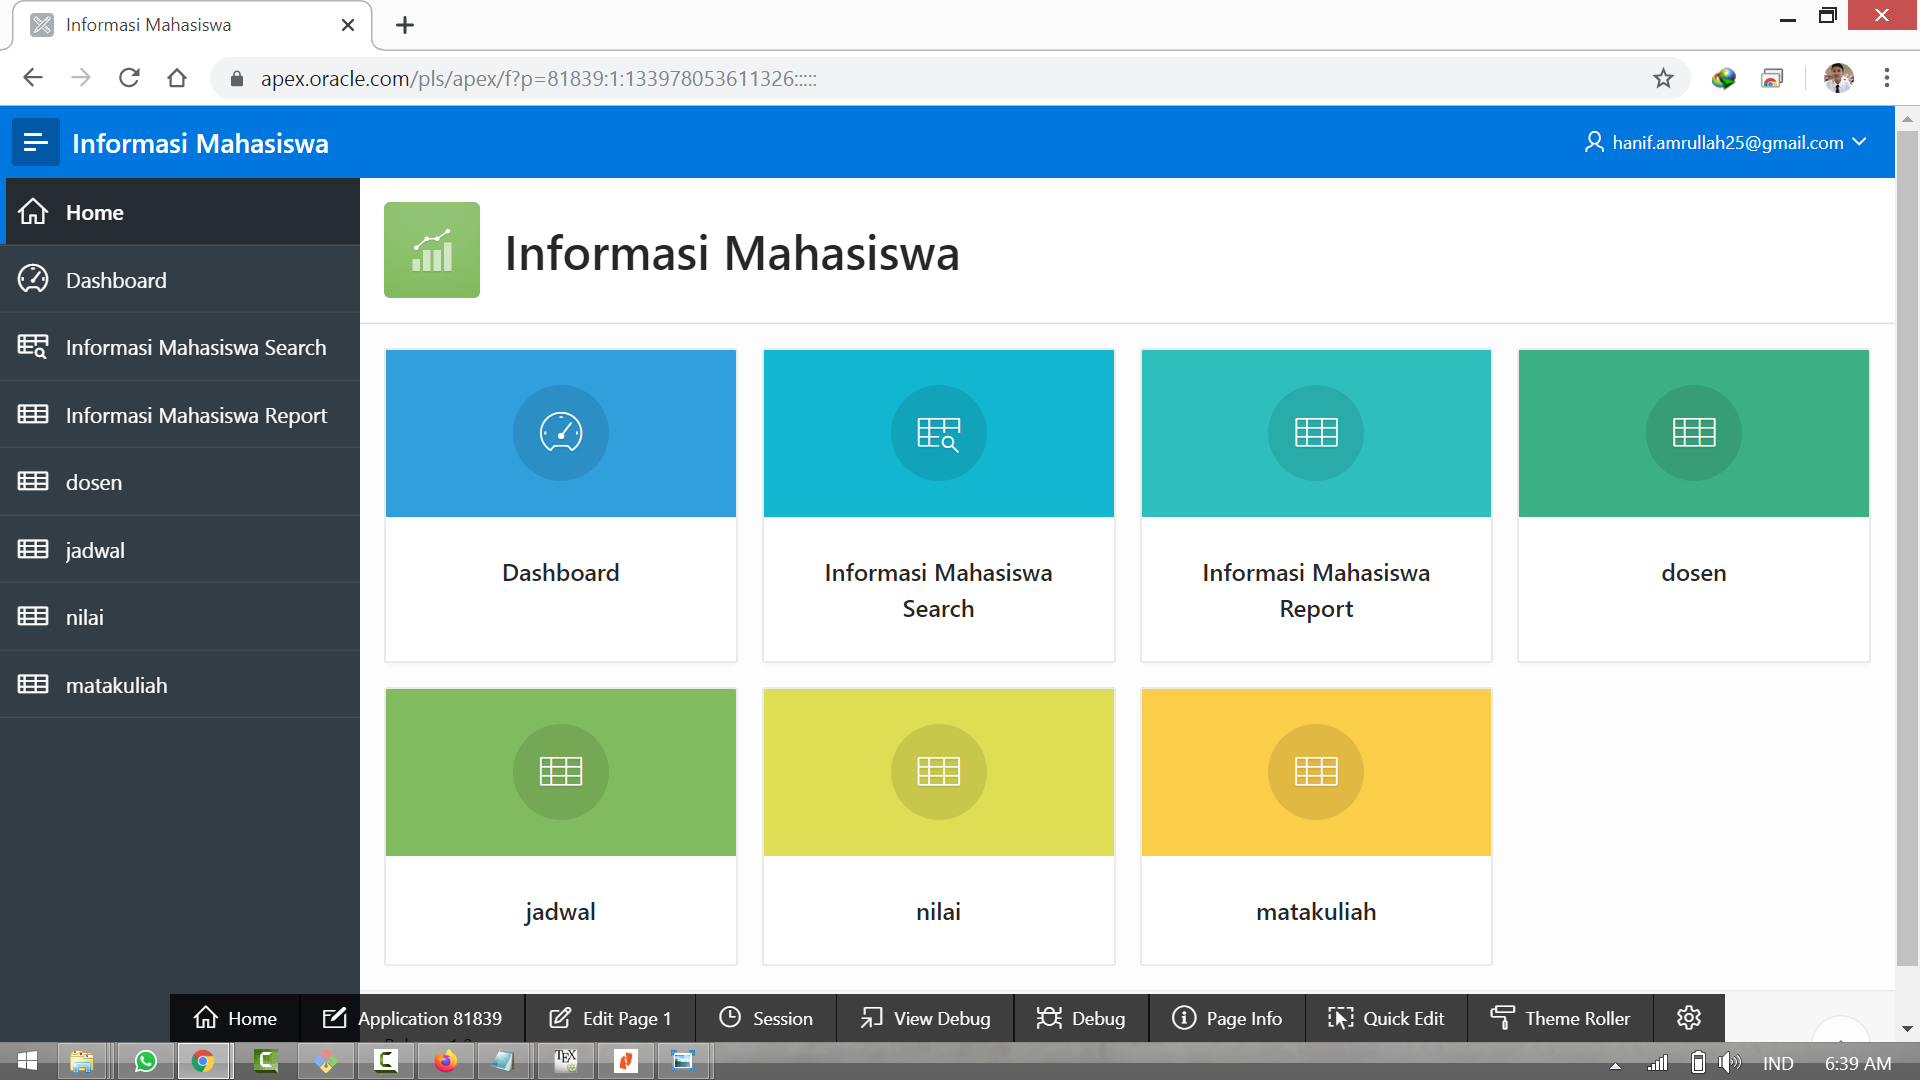
\includegraphics[scale=0.1]{img/b4.png}}
        \centering
        \caption{}
		\label{langkah25}
	\end{figure}
	
\par
link : https://apex.oracle.com/pls/apex/f?p=81839:1:133978053611326:::::\\
workspace : Praktikumbs2\\
id 	  : hanif.amrullah25@gmail.com\\
pw 	  : zxasqw12

	\end{enumerate}
		
\end{document}
